\documentclass[11pt]{article}

\usepackage[utf8]{inputenc}
\usepackage[T1]{fontenc}
\usepackage{lmodern}
\usepackage[spanish, es-noshorthands, es-nodecimaldot, es-tabla]{babel}
\usepackage[margin=2.5cm]{geometry}
\usepackage{amsmath, amssymb, amsthm}
\usepackage{graphicx}
\usepackage{subcaption}
\usepackage{tabularx}
\usepackage{booktabs}
\usepackage{float}
\usepackage[hidelinks]{hyperref}
\usepackage{xurl}

% Margen extra para que los nombres largos de funciones no se salgan de la
% linea.
\setlength{\emergencystretch}{2em}

\graphicspath{{../figuras/}}

\newcolumntype{L}{>{\raggedright\arraybackslash}X}

% Las tablas las escriben los scripts en resultados/. Si una tabla es mas
% ancha que el texto, se reduce para que quepa.
\newsavebox{\cajatabla}
\newcommand{\tabla}[1]{%
  \sbox{\cajatabla}{\input{../resultados/#1.tex}}%
  \ifdim\wd\cajatabla>\linewidth
    \resizebox{\linewidth}{!}{\usebox{\cajatabla}}%
  \else
    \usebox{\cajatabla}%
  \fi}

\title{Tarea 3: Introducción a Series de Tiempo\\
       \large Análisis y Ciencia de Datos}
\author{Herman Andrés Echeverría Rojas\\
        \small Facultad de Ingeniería, Universidad del Istmo de Guatemala}
\date{\today}

\begin{document}
\maketitle

\begin{abstract}
\noindent
Este documento acompaña al repositorio\\
\url{https://github.com/HermanEcheverria/Series-de-Tiempo}.
Todas las figuras y tablas que aparecen aquí las generan los scripts del
repositorio a partir del archivo original \texttt{Online Retail.xlsx} y de las
semillas documentadas en el código.
\end{abstract}

\tableofcontents
\newpage

% Las secciones se agregan conforme se resuelve cada parte.
\section{Parte 0: procesos simulados}
\label{sec:parte0}

Antes de tocar datos reales conviene ver cómo se comportan la ACF y las
pruebas de ruido blanco en procesos donde la respuesta es conocida. Todo lo de
esta sección lo produce \texttt{parte0.py}, con las semillas de
\texttt{semillas.py}; las funciones $r_k$, Ljung--Box y el estimado OLS de
$\phi$ están implementadas a mano en \texttt{series.py} y son las mismas que se
usan con la serie de ventas en las Partes~3 y~4.

\subsection{Inciso 0.1: momentos del AR(1) y de la caminata aleatoria}

Sea $Y_t = c + \phi Y_{t-1} + \varepsilon_t$ con $\varepsilon_t
\overset{\text{iid}}{\sim} \mathcal{N}(0,\sigma^2)$, $|\phi|<1$, y supongamos
que el proceso es débilmente estacionario: $E[Y_t]=\mu$ y
$\operatorname{Var}(Y_t)=\gamma_0$ para todo $t$.

\paragraph{Media.} Tomando esperanza en ambos lados y usando
$E[\varepsilon_t]=0$:
\[
  \mu = E[Y_t] = c + \phi\,E[Y_{t-1}] + E[\varepsilon_t] = c + \phi\mu
  \quad\Longrightarrow\quad
  \mu(1-\phi) = c
  \quad\Longrightarrow\quad
  E[Y_t] = \frac{c}{1-\phi}.
\]
La división es válida porque $|\phi|<1$ implica $\phi\neq 1$.

\paragraph{Varianza.} $Y_{t-1}$ depende solo de
$\varepsilon_{t-1},\varepsilon_{t-2},\dots$, así que es independiente de
$\varepsilon_t$ y la covarianza entre ambos es cero. La constante $c$ no
aporta varianza. Entonces
\[
  \gamma_0 = \operatorname{Var}(c + \phi Y_{t-1} + \varepsilon_t)
  = \phi^2 \operatorname{Var}(Y_{t-1}) + \operatorname{Var}(\varepsilon_t)
  + 2\phi\operatorname{Cov}(Y_{t-1},\varepsilon_t)
  = \phi^2\gamma_0 + \sigma^2,
\]
donde se usó $\operatorname{Var}(Y_{t-1})=\operatorname{Var}(Y_t)=\gamma_0$.
Despejando,
\[
  \operatorname{Var}(Y_t) = \gamma_0 = \frac{\sigma^2}{1-\phi^2},
\]
que es positiva y finita justamente porque $\phi^2<1$.

\paragraph{Autocorrelación.} Para $k\geq 1$, $Y_{t-k}$ depende solo de choques
anteriores a $t-k+1$, así que $\operatorname{Cov}(\varepsilon_t, Y_{t-k})=0$ y
la constante no covaría con nada:
\[
  \gamma_k = \operatorname{Cov}(Y_t, Y_{t-k})
  = \operatorname{Cov}(c + \phi Y_{t-1} + \varepsilon_t,\; Y_{t-k})
  = \phi\,\operatorname{Cov}(Y_{t-1}, Y_{t-k})
  = \phi\,\gamma_{k-1}.
\]
El último paso usa la estacionariedad: la covarianza entre $Y_{t-1}$ y
$Y_{t-k}$ solo depende de su separación, $k-1$. Iterando la recursión desde
$\gamma_0$ se obtiene $\gamma_k = \phi^k\gamma_0$, y por lo tanto
\[
  \rho_k = \frac{\gamma_k}{\gamma_0} = \phi^k .
\]

\paragraph{Caminata aleatoria.} Con $\phi=1$, $c=0$ y $Y_0=0$, sustituyendo
hacia atrás,
\[
  Y_t = Y_{t-1} + \varepsilon_t = Y_{t-2} + \varepsilon_{t-1} + \varepsilon_t
  = \dots = Y_0 + \sum_{i=1}^{t}\varepsilon_i = \sum_{i=1}^{t}\varepsilon_i .
\]
Los $\varepsilon_i$ son independientes, así que la varianza de la suma es la
suma de las varianzas:
\[
  \operatorname{Var}(Y_t) = \sum_{i=1}^{t}\operatorname{Var}(\varepsilon_i)
  = t\sigma^2 .
\]
La media sí es constante ($E[Y_t]=0$), pero la varianza crece linealmente con
$t$: depende del momento en que se observa, y eso viola directamente la
condición $\operatorname{Var}(Y_t)=\sigma^2$ para todo $t$ de la
estacionariedad débil. Dicho de otra forma, la fórmula
$\sigma^2/(1-\phi^2)$ explota cuando $\phi\to 1$: no existe una varianza
estacionaria a la cual converger. Tampoco la autocorrelación es función solo
del rezago: $\operatorname{Corr}(Y_t,Y_{t-k}) = \sqrt{(t-k)/t}$, que depende
de $t$.

\subsection{Inciso 0.2: simulación del AR(1)}

La función \texttt{simular\_ar1} genera $200+300$ pasos de un AR(1) con $c=0$
y $\sigma=1$ a partir de $Y_0=0$ y descarta los primeros 200. Con $|\phi|<1$
el efecto del valor inicial decae como $\phi^t$; a los 200 pasos, incluso con
$\phi=0.9$, queda $0.9^{200}\approx 7\times10^{-10}$ del valor inicial, así
que la serie que se conserva ya está en su distribución estacionaria. Con
$\phi=1$ eso no funciona: la serie conservada es $Y_t = Y_{200} +
\sum_{i=201}^{t}\varepsilon_i$, una caminata aleatoria que arranca en
$Y_{200}$ en lugar de 0, y la varianza sigue creciendo sin límite. Pero el
punto de arranque no afecta a $r_k$: sumar una constante a toda la serie mueve
también a $\bar y$ y deja intactas las desviaciones $y_t-\bar y$, que son lo
único que entra en la fórmula. Por eso descartar o no los 200 pasos no cambia
en nada los resultados de $r_k$ para la caminata.

La figura~\ref{fig:p0_realizaciones} muestra una realización de cada
proceso. Con $\phi=0$ la serie no tiene ninguna inercia; con $\phi=0.5$
aparecen rachas cortas; con $\phi=0.9$ la serie pasa decenas de pasos de un
mismo lado de cero, aunque siempre regresa; y con $\phi=1$ nunca regresa: se
aleja de su origen (nótese que arranca en $Y_{200}\neq0$) y lo que en un AR
estacionario serían fluctuaciones aquí parece una tendencia.

\begin{figure}[H]
  \centering
  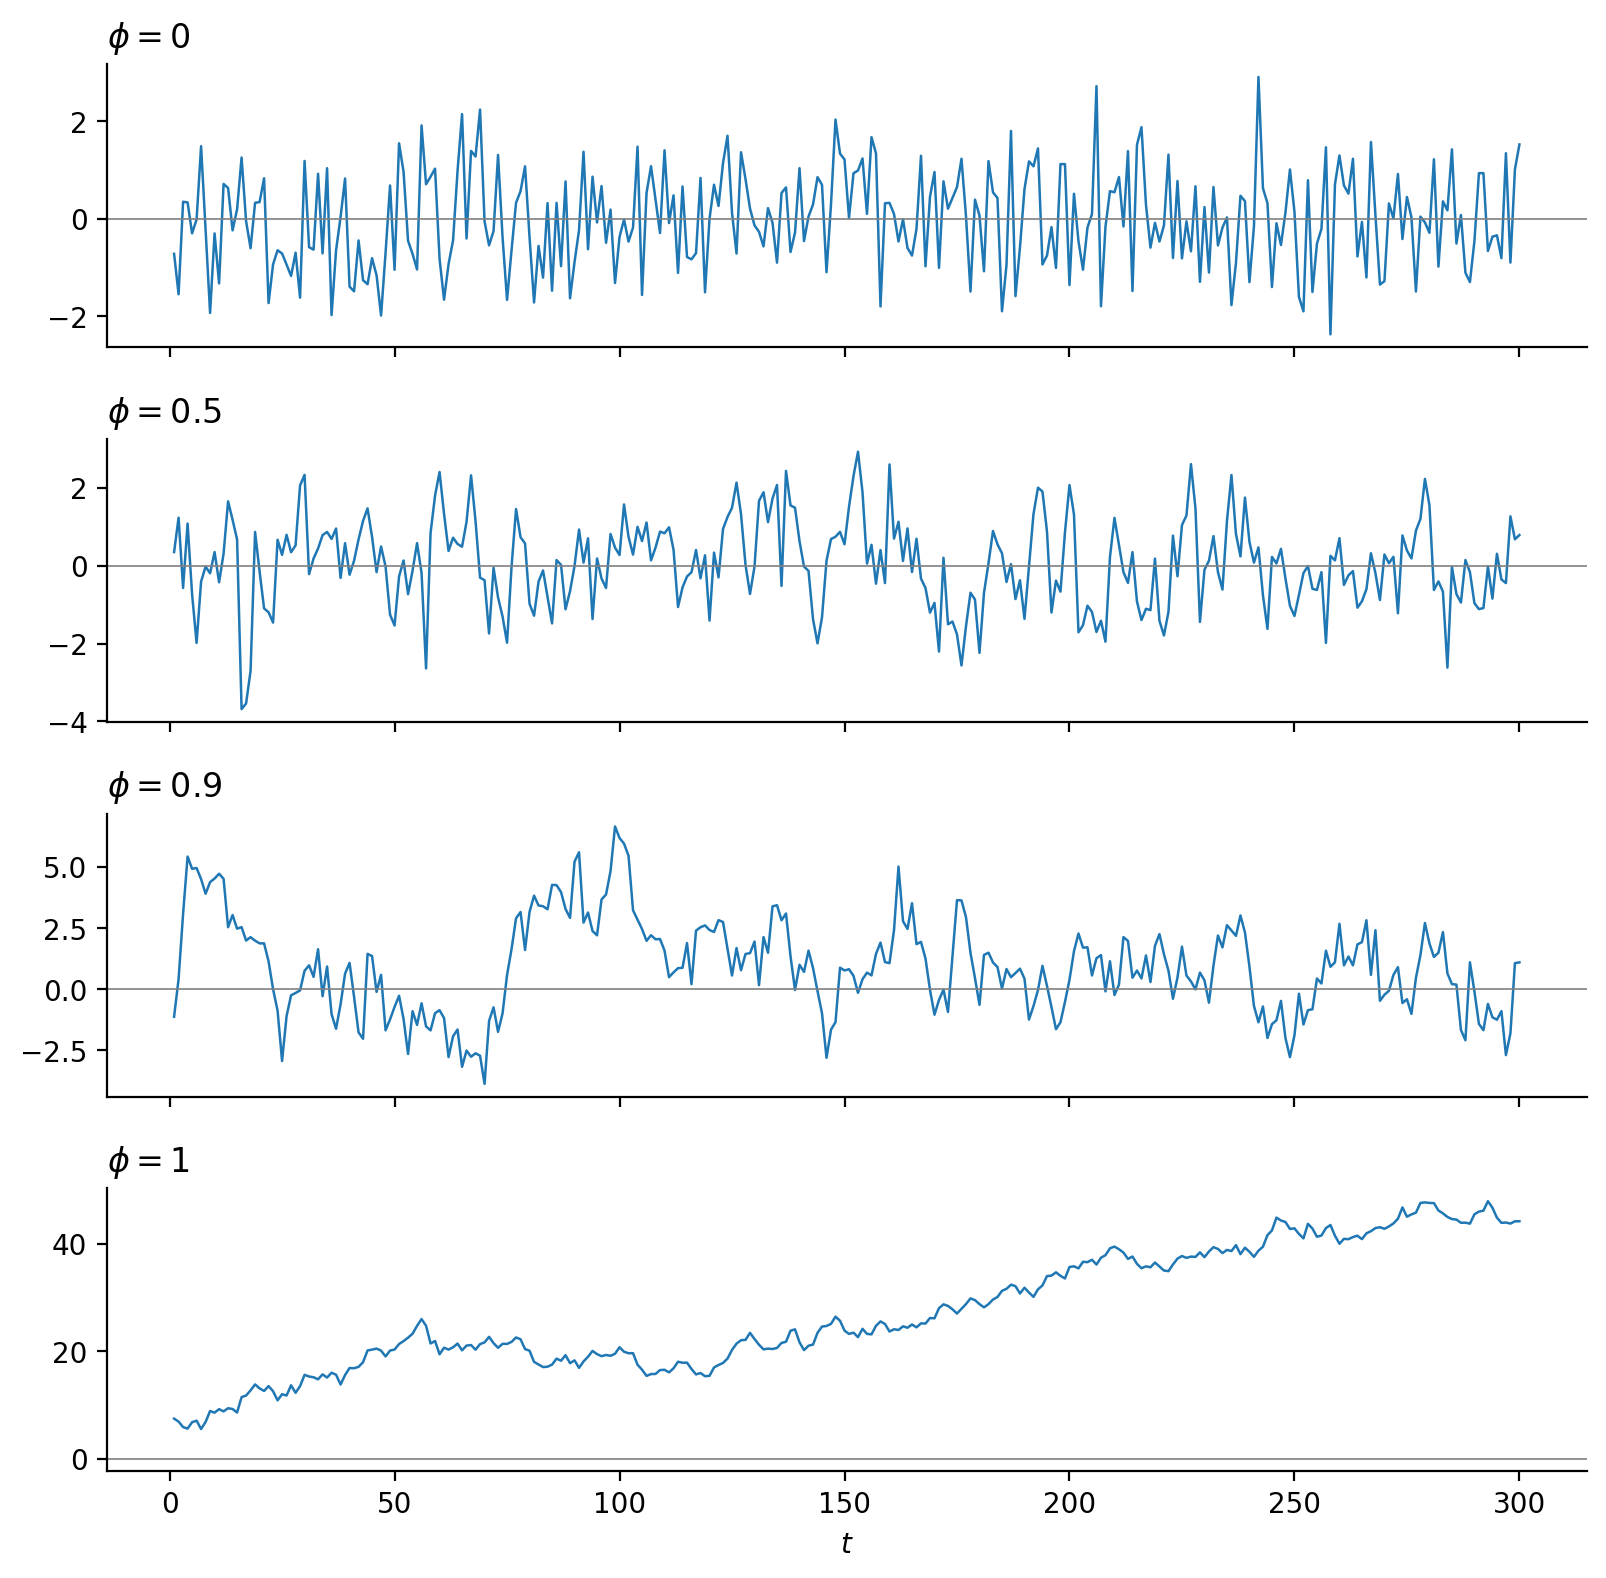
\includegraphics[width=0.85\textwidth]{p0_realizaciones_ar1.png}
  \caption{Una realización de 300 pasos de cada AR(1), después de descartar
  200 pasos de arranque. La escala vertical cambia entre paneles: la varianza
  estacionaria $1/(1-\phi^2)$ vale 1, 1.33 y 5.26 para $\phi=0,0.5,0.9$, y no
  existe para $\phi=1$.}
  \label{fig:p0_realizaciones}
\end{figure}

La tabla~\ref{tab:p0_ar1} resume las 5\,000 réplicas por escenario. Cada
celda es el promedio sobre réplicas y, entre paréntesis, su error estándar
$s/\sqrt{5000}$. La tasa de rechazo es la fracción de réplicas en que
$|r_1|>1.96/\sqrt{300}=0.113$, es decir, en que la prueba de retardo 1 de la
Tarea~2 declara que la serie no es ruido blanco.

\begin{table}[H]
  \centering
  \small
  \begin{tabular}{cccccc}
\toprule
$\phi$ & $\bar r_1$ & $\bar r_5$ & $\phi^5$ & Rechazo $|r_1|>1.96/\sqrt{n}$ & $\bar{\hat\phi}_{\text{OLS}}$ \\
\midrule
0 & -0.002 (0.001) & -0.003 (0.001) & 0.000 & 0.046 (0.003) & -0.002 (0.001) \\
0.5 & 0.491 (0.001) & 0.020 (0.001) & 0.031 & 1.000 (0.000) & 0.492 (0.001) \\
0.9 & 0.884 (0.000) & 0.534 (0.001) & 0.590 & 1.000 (0.000) & 0.887 (0.000) \\
1 & 0.976 (0.000) & 0.883 (0.001) & 1.000 & 1.000 (0.000) & 0.982 (0.000) \\
\bottomrule
\end{tabular}

  \caption{AR(1) con $n=300$ y 5\,000 réplicas por valor de $\phi$. Promedio
  (error estándar).}
  \label{tab:p0_ar1}
\end{table}

\subsection{Inciso 0.3: lo que dice la tabla}

\paragraph{Ruido blanco.} Con $\phi=0$ la prueba rechaza en el 4.62\% de las
réplicas, con error estándar de 0.30 puntos: está a poco más de un error
estándar del 5\% nominal, que es lo esperado. La prueba está construida
precisamente para equivocarse un 5\% de las veces cuando la hipótesis nula es
cierta, y aquí la nula es cierta por construcción. Que quede un poco por debajo
de 5\% tiene además una razón teórica: bajo ruido blanco, $E[r_1]\approx-1/n$
y $\operatorname{Var}(r_1)\approx (n-1)/(n(n+2))$, ligeramente menor que la
$1/n$ con que se dibujan las bandas, así que la tasa exacta ronda 4.9\%. El
$\bar r_1=-0.0023$ observado también es compatible con $-1/300=-0.0033$.

\paragraph{Caminata aleatoria.} La teoría estacionaria diría $\rho_5=\phi^5=1$,
pero el promedio de $r_5$ es 0.883. No es un error de simulación (el error
estándar es 0.001): para una caminata aleatoria la ACF muestral está
fuertemente sesgada hacia abajo. La razón es que $r_k$ mide desviaciones
respecto a $\bar y$, y en una caminata $\bar y$ es una media que no
representa a ningún tramo de la serie: la serie se pasa largos periodos de un
lado y luego del otro. Además el denominador usa los $n$ términos y el
numerador solo $n-k$. De hecho, la fórmula $\rho_k=\phi^k$ ni siquiera
aplica, porque la derivación del inciso 0.1 supuso estacionariedad. Lo que sí
se ve es la huella visual que menciona el enunciado: la ACF de la caminata
baja muy despacio ($\bar r_1=0.976$, $\bar r_5=0.883$), mientras que con
$\phi=0.5$ el valor ya cayó a casi cero en el rezago 5. Para los procesos
estacionarios el sesgo de $r_5$ también existe pero es menor: con $\phi=0.9$
se obtiene 0.534 contra $0.9^5=0.590$, y con $\phi=0.5$, 0.020 contra 0.031.

\paragraph{Sesgo del estimado OLS.} El estimado OLS de $\phi$ queda
sistemáticamente por debajo del valor verdadero, y el sesgo crece con $\phi$:
$-0.002$ para $\phi=0$, $-0.008$ para $0.5$, $-0.013$ para $0.9$ y $-0.018$
para $1$, todos varias veces mayores que su error estándar. Es el sesgo de
Hurwicz: en una autorregresión el regresor $y_{t-1}$ no es independiente de
los errores pasados, y la aproximación clásica $E[\hat\phi]-\phi\approx
-(1+3\phi)/n$ da $-0.003$, $-0.008$ y $-0.012$ para los tres casos
estacionarios, muy cerca de lo observado. El estimador es consistente: el
sesgo es de orden $1/n$ y desaparece cuando la muestra crece, aunque con 300
observaciones todavía se nota. En la caminata, la teoría de Dickey--Fuller
dice que $\hat\phi$ converge todavía más rápido (a ritmo $1/n$ en vez de
$1/\sqrt n$) pero con una distribución asimétrica, cargada hacia valores
menores que 1, y eso es lo que se ve en el $0.982$.

\subsection{Inciso 0.4: las dos razones para reprobar}

Ahora $Y_t=m_t+\varepsilon_t$ no tiene ninguna memoria: los $\varepsilon_t$
son independientes y $m_t$ es determinista. La
figura~\ref{fig:p0_sin_memoria} muestra una realización de cada proceso y la
tabla~\ref{tab:p0_sin_memoria} repite la tabla del inciso 0.2 agregando
$\bar r_7$; la primera fila es el ruido blanco del inciso anterior, como
referencia.

\begin{figure}[H]
  \centering
  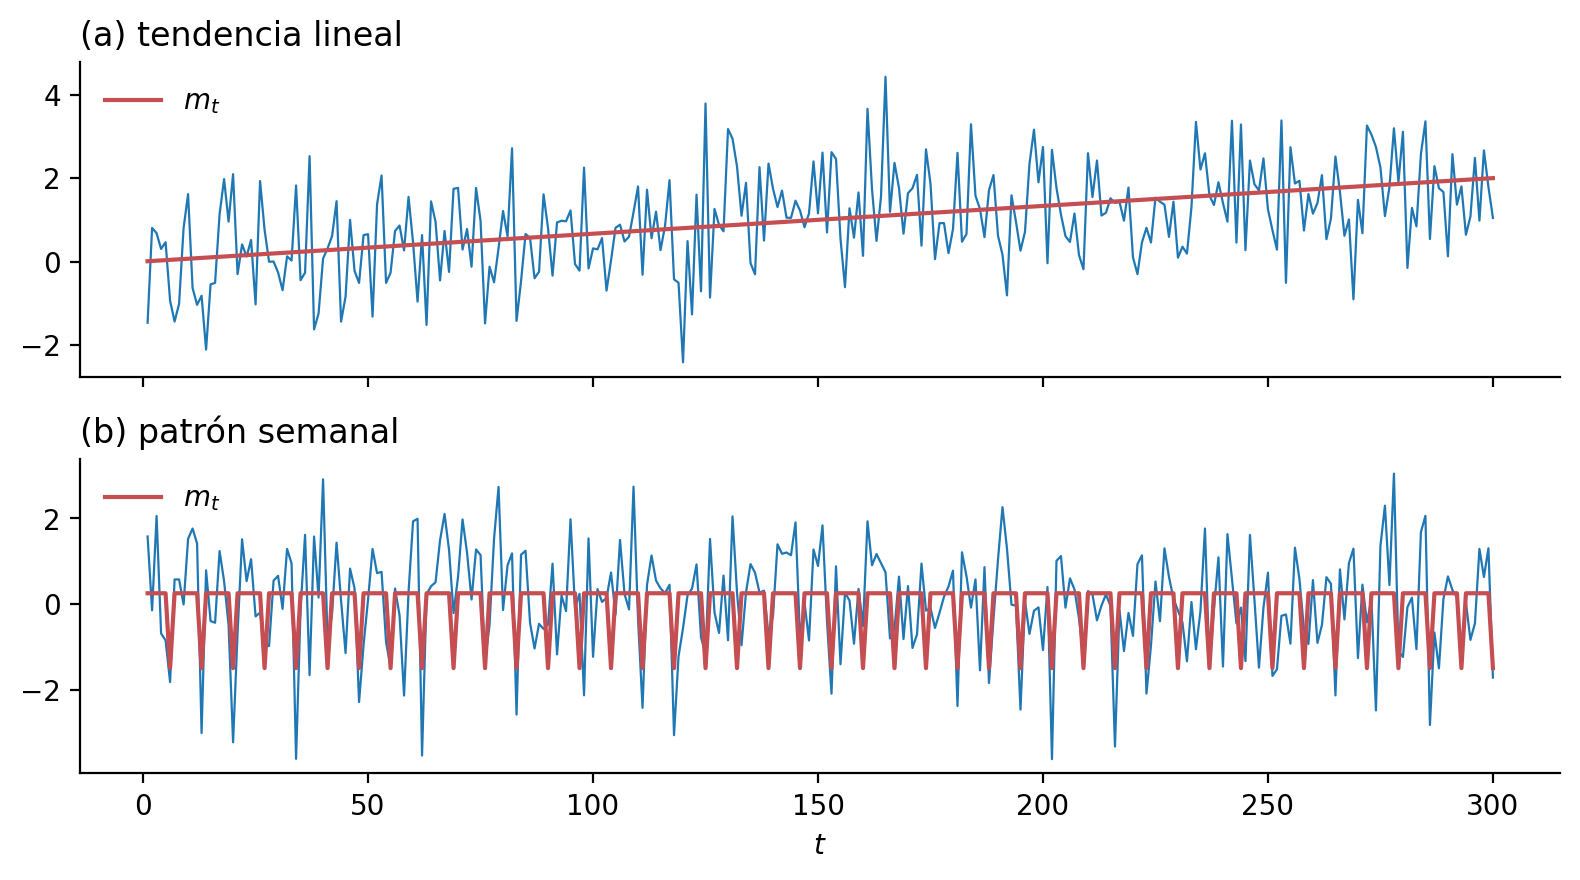
\includegraphics[width=0.85\textwidth]{p0_realizaciones_sin_memoria.png}
  \caption{Procesos sin memoria con media variable. En rojo, la media $m_t$.}
  \label{fig:p0_sin_memoria}
\end{figure}

\begin{table}[H]
  \centering
  \small
  \begin{tabular}{lccccc}
\toprule
Proceso & $\bar r_1$ & $\bar r_5$ & $\bar r_7$ & Rechazo $r_1$ & $\bar{\hat\phi}_{\text{OLS}}$ \\
\midrule
Ruido blanco ($\phi=0$) & -0.002 (0.001) & -0.003 (0.001) & -0.004 (0.001) & 0.046 (0.003) & -0.002 (0.001) \\
(a) Tendencia & 0.246 (0.001) & 0.235 (0.001) & 0.230 (0.001) & 0.986 (0.002) & 0.247 (0.001) \\
(b) Semanal & -0.047 (0.001) & -0.050 (0.001) & 0.266 (0.001) & 0.112 (0.004) & -0.048 (0.001) \\
\bottomrule
\end{tabular}

  \caption{Procesos sin memoria, $n=300$, 5\,000 réplicas. Promedio (error
  estándar).}
  \label{tab:p0_sin_memoria}
\end{table}

\paragraph{La tendencia reprueba sin tener memoria.} La serie con tendencia
rechaza la prueba de retardo 1 en el 98.6\% de las réplicas, y el OLS le
asigna $\hat\phi\approx0.25$ a un proceso cuyo $\phi$ verdadero es cero. Se
puede predecir el número: $m_t$ recorre $[0,2]$ de forma casi uniforme, con
varianza $\approx 4/12=1/3$, y como dos días cercanos tienen casi la misma
$m_t$, la covarianza entre vecinos es esa misma varianza; así $r_k\approx
(1/3)/(1/3+1)=0.25$ para todo rezago pequeño. Eso es exactamente lo que dice
la tabla: $\bar r_1=0.246$, $\bar r_5=0.235$, $\bar r_7=0.230$, una ACF que
casi no decae. Es la razón (2) del enunciado: $\bar y$ no es la media de nadie,
los días del final quedan todos por encima y los del inicio todos por debajo, y
eso se ve como correlación.

\paragraph{El patrón semanal pasa aunque tenga estructura.} La serie semanal
rechaza solo en el 11.2\% de las réplicas, poco más que el ruido blanco, y su
$\bar r_1=-0.047$ es diminuto. De nuevo se puede calcular: sobre un ciclo de 7
días $m_t$ tiene media 0 y varianza $(6\cdot0.25^2+1.5^2)/7=0.375$, pero
la covarianza entre días consecutivos es solo
$(5\cdot0.25^2-2\cdot0.375)/7=-0.0625$, y $r_1\approx-0.0625/1.375=-0.045$.
Toda la estructura está a distancia 7: un domingo se parece al domingo
anterior, no al sábado. Por eso $\bar r_7=0.266$ (la predicción es
$0.375/1.375=0.273$), mientras que $r_1$ y $r_5$ están cerca de cero.

\paragraph{Conexión con RANDU.} Es el mismo fenómeno que con RANDU en la
Tarea~2: RANDU pasaba las pruebas unidimensionales y de pares consecutivos y,
sin embargo, sus ternas caían en solo 15 planos, porque su dependencia vivía en
una combinación de los rezagos 1 y 2 que esas pruebas no miran. La prueba de
retardo 1 solo puede ver estructura en el rezago 1; un proceso con la
dependencia en otro lado (el rezago 7, o una combinación lineal de rezagos)
la pasa sin problema. Pasar una prueba nunca demuestra independencia: solo
dice que en la dirección que esa prueba mira no se encontró nada.

\subsection{Inciso 0.5: la prueba que sí ve}

La tabla~\ref{tab:p0_ljungbox} compara la tasa de rechazo de la prueba de
retardo 1 con la de Ljung--Box al 5\%, con $m=10$ (la recomendación de FPP2
sin estacionalidad) y con $m=6\approx\log(300)=5.7$ (la sugerencia de Tsay).
La implementación propia coincide con
\nolinkurl{statsmodels.stats.diagnostic.acorr_ljungbox} hasta el sexto decimal
en el estadístico y en el valor-$p$; \texttt{parte0.py} lo verifica con un
\texttt{assert} en una réplica de cada proceso.

\begin{table}[H]
  \centering
  \small
  \begin{tabular}{lccc}
\toprule
Proceso & Rechazo $r_1$ & LB $m=10$ & LB $m=6$ \\
\midrule
Ruido blanco ($\phi=0$) & 0.046 (0.003) & 0.053 (0.003) & 0.053 (0.003) \\
(a) Tendencia & 0.986 (0.002) & 1.000 (0.000) & 1.000 (0.000) \\
(b) Semanal & 0.112 (0.004) & 0.956 (0.003) & 0.209 (0.006) \\
\bottomrule
\end{tabular}

  \caption{Tasa de rechazo al 5\% sobre 5\,000 réplicas, $n=300$. Promedio
  (error estándar).}
  \label{tab:p0_ljungbox}
\end{table}

Con ruido blanco las dos versiones de Ljung--Box rechazan alrededor del 5\%
(5.3\%), como deben. Con la tendencia rechazan siempre, igual que la prueba de
retardo 1: ahí la estructura se ve en todos los rezagos.

El cambio está en el patrón semanal. Ljung--Box con $m=10$ lo rechaza en el
95.6\% de las réplicas, contra el 11.2\% de la prueba de retardo 1, porque
$Q(10)$ suma $r_k^2$ para $k=1,\dots,10$ y eso incluye el $r_7\approx0.27$
que la prueba de retardo 1 no mira; elevado al cuadrado y multiplicado por
$n(n+2)/(n-7)$, ese solo término aporta alrededor de 22 al estadístico, cuando
el valor crítico de una $\chi^2_{10}$ al 5\% es 18.3. En cambio, con $m=6$ la
tasa cae a 20.9\%: seis rezagos no llegan al 7, así que $Q(6)$ es casi tan
ciego como la prueba de retardo 1. Esta es la comparación que pedía el
enunciado entre las dos reglas para escoger $m$, y la lección es que $m$ tiene
que cubrir al menos el periodo estacional; por eso FPP2 recomienda $m=2s$
cuando hay estacionalidad. Con datos diarios de una tienda, la regla
$m\approx\log n$ por sí sola no es suficiente.

\section{Parte 1: limpieza}
\label{sec:parte1}

La limpieza vive en \texttt{limpiar.py} y la reproduce \texttt{parte1.py}. El
archivo se carga con \texttt{datos.cargar\_crudo()}, que lee
\texttt{InvoiceNo}, \texttt{StockCode} y \texttt{CustomerID} como texto. El
enunciado sugiere hacerlo y pide averiguar por qué; leyendo el archivo sin
indicarle tipos a pandas se ve el problema en cada columna:
\begin{itemize}
  \item \texttt{InvoiceNo} queda como una columna con 532\,618 enteros
    (\texttt{536365}) y 9\,291 cadenas (\texttt{C536379}) revueltos. Entonces
    \texttt{str.startswith('C')} devuelve \texttt{NaN}, no \texttt{False}, en
    todas las filas numéricas, y cualquier filtro de cancelaciones construido
    así falla en silencio.
  \item \texttt{StockCode} mezcla 487\,036 códigos numéricos con 54\,873
    alfanuméricos (\texttt{85123A}, \texttt{POST}). Una regla sobre el texto
    del código, como ``empieza con cinco dígitos'', se salta todas las filas
    que pandas convirtió en enteros.
  \item \texttt{CustomerID} tiene faltantes, y como una columna entera de
    pandas no admite \texttt{NaN}, se convierte a \texttt{float}:
    \texttt{17850.0}. Un identificador no es una cantidad: no se suma ni se
    promedia, y no debería tener decimales.
\end{itemize}

\subsection{Inciso 1.1: el archivo crudo}

\begin{table}[H]
  \centering
  \small
  \tabla{p1_resumen}
  \caption{Tamaño del archivo original, antes de limpiar.}
  \label{tab:p1_resumen}
\end{table}

El archivo tiene 541\,909 líneas de 25\,900 facturas, 4\,070 códigos de
producto y 4\,372 clientes (tabla~\ref{tab:p1_resumen}). El 24.9\% de las
filas no tiene \texttt{CustomerID}. El número de productos depende de cómo se
cuente: 117 códigos aparecen también en minúscula (\texttt{85123a} junto a
\texttt{85123A}), y unificándolos quedan 3\,958.

\subsection{Inciso 1.2: caso por caso}

La tabla~\ref{tab:p1_casos} cuenta cada caso sobre los datos crudos, sin
aplicar ninguna otra regla, y resume la decisión. El monto es la suma con
signo de $\texttt{Quantity}\times\texttt{UnitPrice}$ de esas filas.

\begin{table}[H]
  \centering
  \small
  \tabla{p1_casos}
  \caption{Casos del inciso 1.2 sobre los datos crudos. Un caso puede
  traslapar con otro; el efecto conjunto está en la bitácora
  (tabla~\ref{tab:p1_bitacora}).}
  \label{tab:p1_casos}
\end{table}

\paragraph{(a) Duplicados exactos: se van.} Hay 5\,268 filas idénticas en las
ocho columnas a otra fila anterior: misma factura, mismo producto, misma
cantidad y mismo minuto. Una factura que de verdad incluyera dos veces el
mismo artículo lo registraría como una línea con la cantidad sumada; dos
líneas idénticas son una doble captura. Se conserva la primera. Representan
\pounds21\,741.

\paragraph{(b) Facturas que no empiezan con un dígito.} Hay dos prefijos. El
\texttt{C} marca 9\,288 cancelaciones, todas con cantidad negativa: \emph{se
quedan}, porque la venta neta diaria las define como líneas que restan el día
en que ocurren. El \texttt{A} aparece en tres facturas del 12 de agosto de 2011
con el código \texttt{B}, ``Adjust bad debt'', por $+11\,062$ y dos veces
$-11\,062$ libras: \emph{se van}, porque son asientos contables de deuda
incobrable, no ventas ni devoluciones de mercancía.

\paragraph{(c) Códigos que no son productos.} La tabla~\ref{tab:p1_codigos}
lista todos los códigos que no empiezan con cinco dígitos. No todos son
iguales:
\begin{itemize}
  \item \emph{Se van} los cargos que no son mercancía: envío (\texttt{POST},
    \texttt{DOT}, \texttt{C2}), comisiones (\texttt{AMAZONFEE},
    \texttt{CRUK}), cargos bancarios, muestras (\texttt{S}), el ajuste de
    deuda \texttt{B} y los vales de regalo \texttt{gift\_0001\_*}, que son
    dinero adelantado y se contarían dos veces cuando se canjearan. El caso
    que más pesa es \texttt{AMAZONFEE}: 32 de sus 34 filas son
    ``cancelaciones'' de hasta \pounds17\,836, que en realidad son la
    comisión que cobra Amazon. Dejarlas habría restado \pounds221\,521 de
    ventas que nunca se devolvieron.
  \item \emph{Se quedan} los \texttt{DCGS...} (artículos de la tienda
    \emph{dotcom}, como bolsas de fiesta o collares) y \texttt{PADS}, que sí
    son productos aunque su código no tenga cinco dígitos.
  \item \emph{Se quedan} también \texttt{D} (descuento) y \texttt{M}
    (ajuste manual). No son productos, pero corrigen el precio de mercancía
    que sí se vendió: un descuento reduce lo que la tienda cobró. El inciso
    1.4 muestra qué pasa si se quitan: la factura 556444 cobró por error 60
    canastas a \pounds649.50 cada una, y la corrección es la línea
    \texttt{M} de la cancelación C556445. Si se quitaran las \texttt{M}, la
    serie se quedaría con una venta fantasma de \pounds38\,970.
  \item \emph{Se transforman} los 117 códigos en minúscula, que se pasan a
    mayúscula.
\end{itemize}

\begin{table}[H]
  \centering
  \small
  \tabla{p1_codigos}
  \caption{Códigos que no empiezan con cinco dígitos, en los datos crudos. La
  columna de cancelación es el porcentaje de sus filas en facturas \texttt{C}.}
  \label{tab:p1_codigos}
\end{table}

\paragraph{(d) Precios iguales a cero o negativos: se van.} Los dos precios
negativos son las líneas de deuda incobrable del caso (b). Los 2\,515 precios
en cero no aportan nada a la venta (su monto es exactamente cero), y casi
todos son movimientos de inventario sin cliente: 1\,336 tienen cantidad
negativa (caso e) y, de las que tienen cantidad positiva, solo 40 tienen
cliente, probablemente obsequios. Para la serie da igual quitarlos o no; se
quitan para que no inflen la frecuencia de compra en la Parte 6.

\paragraph{(e) Cantidades negativas que no son cancelaciones: se van.} Son
1\,336 filas, todas con precio cero y ninguna con cliente. Su descripción lo
explica: vacía (862), ``check'' (123), ``damaged'' o ``damages'' (103),
``?'' (41), ``sold as set on dotcom'', ``thrown away'', ``wet damaged'',
``missing''\dots{} Son ajustes de inventario por mercancía dañada, perdida o
reetiquetada, no devoluciones de clientes.

\paragraph{(f) Filas sin \texttt{CustomerID}: depende.} Para la serie de
ventas \emph{se quedan}: una venta sin cliente identificado sigue siendo
dinero que entró a la tienda. Después de la limpieza son el 24.8\% de las
filas y el 15.4\% de la venta neta (\pounds1.50 millones), casi todas del
Reino Unido; quitarlas bajaría el nivel de la serie y, si su peso cambia con
el tiempo, también su forma. Para la Parte 6 \emph{se van}, porque el RFM
necesita saber quién compró. Por eso \texttt{limpiar} tiene el argumento
\texttt{requiere\_cliente}.

\subsection{Inciso 1.3: bitácora de limpieza}

Las reglas se aplican en el orden de la tabla~\ref{tab:p1_bitacora}. La
columna ``Sola'' cuenta las filas que la regla quitaría aplicada sobre los
datos crudos; ``En orden'' cuenta las que realmente quita después de las
anteriores. El monto corresponde a las filas que quita en orden: el neto es la
suma con signo y el absoluto, la suma de $|\texttt{Quantity}\times
\texttt{UnitPrice}|$. La regla 6 solo se aplica para la Parte 6.

\begin{table}[H]
  \centering
  \small
  \tabla{p1_bitacora}
  \caption{Bitácora de limpieza, en el orden en que se aplican las reglas.}
  \label{tab:p1_bitacora}
\end{table}

El orden sí cambia los conteos. La regla 5 no quita ninguna fila en orden,
pero aplicada sola quitaría 1\,336: todas las cantidades negativas sin
cancelación tienen precio cero, así que la regla 4 ya las eliminó. Si el orden
fuera el inverso, la regla 5 se llevaría 1\,336 filas y la 4, 1\,336 menos.
Del mismo modo, la regla 3 quita 2\,293 filas y no 2\,297 porque las tres
líneas \texttt{B} ya cayeron con el prefijo \texttt{A} y una más era
duplicado; y la regla 4 quita 2\,499 y no 2\,517 porque los dos precios
negativos ya cayeron con el prefijo \texttt{A}, cinco eran duplicados y once
tenían un código que no es producto.
Ninguna de estas diferencias cambia el resultado final: las reglas solo
deciden a qué renglón de la bitácora se le atribuye cada fila.

Para la serie de ventas (reglas 1 a 5) quedan 531\,846 filas con una venta
neta total de \pounds9\,696\,590; 8\,989 de esas filas son cancelaciones que
suman $-$\pounds628\,382. Para el RFM (reglas 1 a 6) quedan 400\,190 filas.

\subsection{Inciso 1.4: las seis líneas más grandes}

La tabla~\ref{tab:p1_top6} muestra las seis líneas con mayor
$|\texttt{Quantity}\times\texttt{UnitPrice}|$ en los datos crudos. Son tres
pares venta--cancelación.

\begin{table}[H]
  \centering
  \footnotesize
  \tabla{p1_top6}
  \caption{Las seis líneas con mayor monto absoluto antes de limpiar.
  ``¿Sobrevive?'' indica si la línea sigue en los datos limpios.}
  \label{tab:p1_top6}
\end{table}

\begin{itemize}
  \item \textbf{Paper Craft, Little Birdie (cliente 16446).} El 9 de diciembre
    de 2011 a las 9:15 la factura 581483 vende 80\,995 unidades a \pounds2.08,
    \pounds168\,470 en una sola línea, y doce minutos después la C581484 la
    cancela completa. El cliente solo tiene otra compra en todo el año: dos
    artículos por \pounds2.90 en mayo. Es casi seguro un error de captura,
    corregido de inmediato.
  \item \textbf{Medium Ceramic Top Storage Jar (cliente 12346).} El 18 de
    enero de 2011 la factura 541431 vende 74\,215 frascos a \pounds1.04
    (\pounds77\,184), y dieciséis minutos después la C541433 la cancela. Es
    la única actividad del cliente en todo el archivo, así que su venta neta
    total es cero; vuelve a aparecer en la Parte 6 como un cliente con
    $M\leq 0$.
  \item \textbf{Picnic Basket Wicker 60 Pieces (cliente 15098).} El 10 de
    junio de 2011 la secuencia completa es: 556442 vende 60 canastas
    pequeñas a \pounds4.95 (\pounds297); 556444 cobra 60 unidades a
    \pounds649.50, que es el precio del juego de 60 piezas, no de una canasta
    (\pounds38\,970); C556445 lo corrige con una línea \texttt{Manual} de
    $-$\pounds38\,970; 556446 cobra el juego correcto, una unidad a
    \pounds649.50; y C556448 cancela las canastas pequeñas. Lo que el cliente
    compró en realidad fue un juego de \pounds649.50.
\end{itemize}

\paragraph{¿Las resuelve la limpieza?} No: las seis sobreviven, y está bien
que sobrevivan. Ninguna regla las identifica como errores (son productos
reales, con precio positivo y con cliente), y quitar una sola mitad del par
sería peor que dejar las dos. Si una regla quitara la venta de 80\,995
unidades por ``atípica'', la cancelación quedaría huérfana y restaría
\pounds168\,470 ese día. Por la misma razón la regla de códigos no quita la
línea \texttt{M}: quitarla dejaría la venta de \pounds38\,970.

\paragraph{¿Las resuelve el neteo por día?} Sí, porque en los tres casos la
venta y su corrección ocurren el mismo día, con minutos de diferencia. En la
venta neta del 18 de enero el par del frasco suma exactamente cero; la del 10
de junio recibe del cliente 15098 exactamente los \pounds649.50 que compró; y
el par del 9 de diciembre suma cero (además, la Parte 2 descarta ese día por
incompleto). La serie diaria es inmune a estos errores siempre que se corrijan
el mismo día. Un análisis por cliente o por factura no lo es: en la Parte 6
cada una de estas facturas cuenta como una compra para la frecuencia, aunque
el monto neto sea cero.

\section{Parte 2: el calendario}
\label{sec:parte2}

La serie se construye en \texttt{calendario.py}: se suma
$\texttt{Quantity}\times\texttt{UnitPrice}$ por día sobre los datos de
\texttt{limpiar(df)} (reglas 1 a 5, con cancelaciones restando y con las
ventas sin cliente) y se lleva al calendario completo. Las tablas y figuras de
esta sección las genera \texttt{parte2.py}.

\subsection{Inciso 2.1: la serie de venta neta diaria}

\begin{table}[H]
  \centering
  \small
  \tabla{p2_resumen}
  \caption{Días calendario y días con transacciones.}
  \label{tab:p2_resumen}
\end{table}

Entre el 1 de diciembre de 2010 y el 9 de diciembre de 2011, contando ambos,
hay 374 días calendario, y en 305 hubo al menos una transacción
(tabla~\ref{tab:p2_resumen}). Es decir, en 69 días (el 18\%) la tienda no
registró nada. La figura~\ref{fig:p2_serie} muestra la serie en los días
abiertos. Los cierres entre semana están marcados con una cruz sobre el eje;
los sábados no se marcan porque ocurren todas las semanas.

\begin{figure}[H]
  \centering
  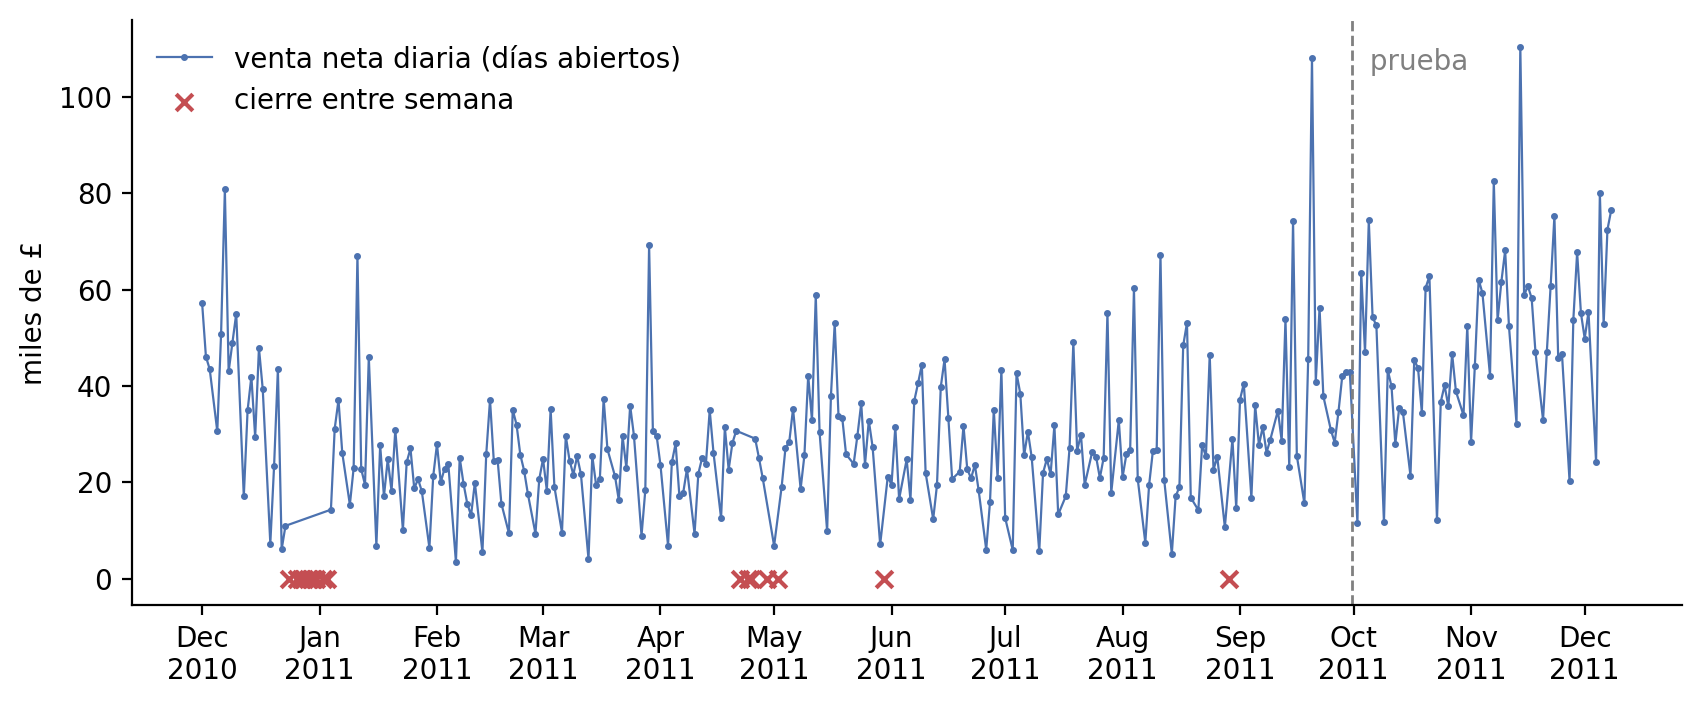
\includegraphics[width=\textwidth]{p2_serie_diaria.png}
  \caption{Venta neta diaria en los días abiertos, del 1 de diciembre de 2010
  al 8 de diciembre de 2011. La línea une días abiertos consecutivos, así que
  salta por encima de los sábados y de los cierres. La línea punteada separa
  el entrenamiento (hasta el 30 de septiembre) de la prueba.}
  \label{fig:p2_serie}
\end{figure}

La figura ya anticipa lo que se va a modelar en las siguientes partes: un
nivel de alrededor de \pounds20--30 mil diarios entre enero y agosto, un
crecimiento fuerte desde septiembre (la temporada navideña de una tienda de
regalos que vende a mayoristas) y mucha variación de un día a otro, con picos
aislados de más de \pounds100 mil.

\subsection{Inciso 2.2: los días sin transacciones}

\paragraph{Los sábados.} 53 de los 69 días faltantes son sábados: \emph{todos}
los sábados del periodo. No hay ni una sola transacción en sábado en todo el
año, así que la tienda no abre ese día. En cambio sí abre los domingos.

\paragraph{Los otros 16.} La tabla~\ref{tab:p2_cierres} los lista y los
clasifica usando el calendario de \emph{bank holidays} de Inglaterra y Gales.

\begin{table}[H]
  \centering
  \small
  \tabla{p2_cierres}
  \caption{Días entre semana (sin contar sábados) sin ninguna transacción.}
  \label{tab:p2_cierres}
\end{table}

\begin{itemize}
  \item \textbf{Cierre de Navidad: 9 días}, del viernes 24 de diciembre de
    2010 al lunes 3 de enero de 2011. En 2010 Navidad cayó en sábado y el
    \emph{Boxing Day} en domingo, así que los feriados oficiales se
    trasladaron al lunes 27 y al martes 28; Año Nuevo de 2011 cayó en sábado
    y se trasladó al lunes 3 de enero. Los días que quedan en medio (29, 30 y
    31 de diciembre y el domingo 2 de enero) no son feriados oficiales: la
    tienda simplemente cerró entre fiestas, algo común en un negocio que le
    vende a otros negocios.
  \item \textbf{Pascua: 3 días}, el Viernes Santo (22 de abril), el Domingo de
    Pascua (24 de abril) y el Lunes de Pascua (25 de abril). El domingo no es
    feriado oficial, pero la tienda, que sí abre otros domingos, no abrió
    entre los dos feriados.
  \item \textbf{La boda real: 1 día}, el viernes 29 de abril de 2011, el
    matrimonio del príncipe Guillermo con Catalina Middleton. Es el feriado
    que no se repite: el gobierno lo declaró solo para ese año.
  \item \textbf{Feriados de lunes: 3 días}, el \emph{Early May bank
    holiday} (2 de mayo), el \emph{Spring bank holiday} (30 de mayo) y el
    \emph{Summer bank holiday} (29 de agosto).
\end{itemize}

Todos los feriados oficiales del periodo aparecen como días sin ventas, y
fuera de los sábados no falta ningún otro día: no hay caídas del sistema ni
días perdidos sin explicación.

\paragraph{¿Cuáles son móviles?} Los de Pascua. La Pascua cae el primer
domingo después de la primera luna llena de primavera, así que el Viernes
Santo puede caer en cualquier fecha entre el 20 de marzo y el 23 de abril, y
el Lunes de Pascua tres días después: de un año a otro se mueven hasta cinco
semanas. Por eso
FPP2 dice que son de lo más difícil de modelar con datos diarios: un modelo
con estacionalidad de 7 días o de 365 días no los puede anticipar, porque no
caen a una distancia fija de nada. Los tres feriados de lunes también cambian
de fecha de un año a otro, pero siguen una regla de calendario sencilla
(primer o último lunes del mes), siempre caen en lunes y se conocen con años de
anticipación. La Navidad tiene fecha fija, pero el día de la semana cambia y
con él los traslados, como pasó en 2010. La boda real no se puede modelar con
ningún patrón, porque solo ocurrió una vez.

\subsection{Inciso 2.3: ¿cero o faltante?}

Un día sin transacciones puede ser cualquiera de las dos cosas; depende de
para qué se use la serie.

\paragraph{Cuándo es un cero.} Cuando la pregunta es contable, como cuánto
vendió la tienda en una semana o en un mes, o cuál es la venta promedio por
día calendario. El sábado la caja recibió exactamente cero libras, y sumar la
serie con ceros da el total correcto. Es el uso de la media móvil del inciso
3.1, donde el enunciado pide rellenar con cero: una semana con un feriado sí
vendió menos que una semana normal, y la tendencia debe reflejarlo.

\paragraph{Cuándo es un faltante.} Cuando se modela el comportamiento de la
tienda en los días en que opera: los índices estacionales, la ACF, los
modelos AR y SARIMA y la evaluación del pronóstico. Ahí un cero de sábado no
es una observación de ``un día malo'': no hubo ningún día que observar. Si se
deja como cero, el índice estacional del sábado sería cero (algo que ya se
sabe y no hay que estimar); la media de la serie bajaría un 18\% (69 de 374 días);
aparecería un $r_7$ enorme que no viene de la demanda sino del calendario; y
un pronóstico que acierte ``cero'' cada sábado se vería artificialmente bueno.
Por eso, de aquí en adelante, la serie tiene los días cerrados como faltantes
y los modelos trabajan con una fila por día abierto.

\subsection{Inciso 2.4: el último día}

El 9 de diciembre de 2011 no está completo. Su última factura es de las 12:50
y suma \pounds29\,306 en 49 facturas, cuando un viernes de noviembre o
diciembre vende una mediana de \pounds52\,410. Ningún día anterior del año
registró su última factura antes de las 12:50: los datos se cortaron a
mediodía, probablemente cuando se extrajo el archivo.

Se puede medir qué tan incompleto está. Para cada viernes anterior se calculó
qué fracción de sus ventas se había registrado a las 12:50
(figura~\ref{fig:p2_corte}). La mediana es 54\%, así que el 9 de diciembre
completo habría vendido alrededor de $29\,306/0.54\approx$ \pounds54\,200, en
línea con los viernes anteriores. Es decir, al día le falta casi la mitad.

\begin{figure}[H]
  \centering
  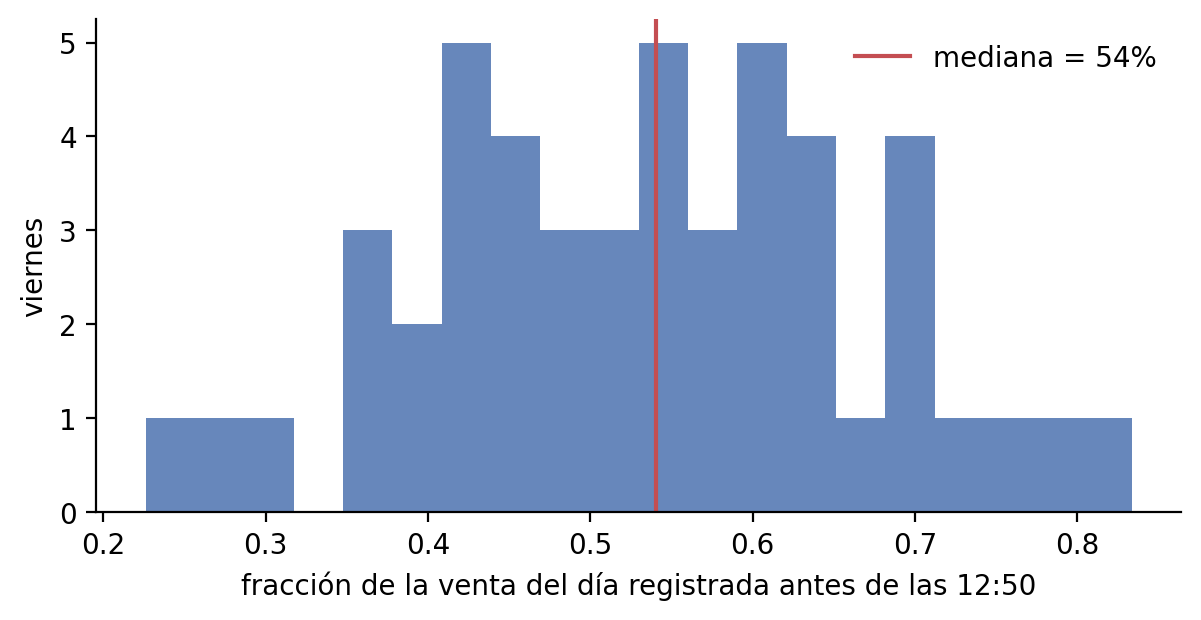
\includegraphics[width=0.7\textwidth]{p2_fraccion_corte.png}
  \caption{Fracción de la venta bruta de cada viernes registrada antes de las
  12:50, la hora de la última factura del 9 de diciembre.}
  \label{fig:p2_corte}
\end{figure}

Se descarta. Dejarlo metería en el último punto de la serie una caída
artificial a la mitad, justo en el día que más pesa al pronosticar, y es
también el día del par venta--cancelación de \pounds168\,470 del inciso 1.4.
Escalarlo por 1/0.54 inventaría un dato con un supuesto sobre el reparto de
las ventas en el día. Como es el último día y no hay nada que interpolar,
quitarlo no le cuesta nada a la serie. La serie de trabajo termina el jueves 8
de diciembre de 2011.

\section{Parte 3: tendencia, estacionalidad y autocorrelación}
\label{sec:parte3}

Los incisos 3.1 y 3.2 forman una descomposición clásica multiplicativa:
\[
  y_t = T_t \times S_t \times R_t,
\]
donde la tendencia $T_t$ se estima con una media móvil, el índice estacional
$S_t$ con el promedio de $y_t/T_t$ por día de la semana, y $R_t$ es lo que
queda. Todo lo genera \texttt{parte3.py}.

\subsection{Inciso 3.1: tendencia}

La media móvil centrada de 7 días es
\[
  MA_t = \frac{1}{7}\sum_{j=-3}^{3} y_{t+j},
\]
calculada sobre el calendario completo con los días cerrados en cero, como
pide el enunciado (aquí el cero es el valor correcto: el inciso 2.3 explica
por qué). Los tres primeros y los tres últimos días no tienen la ventana
completa y quedan sin valor. La figura~\ref{fig:p3_ma} la muestra sobre la
serie.

\begin{figure}[H]
  \centering
  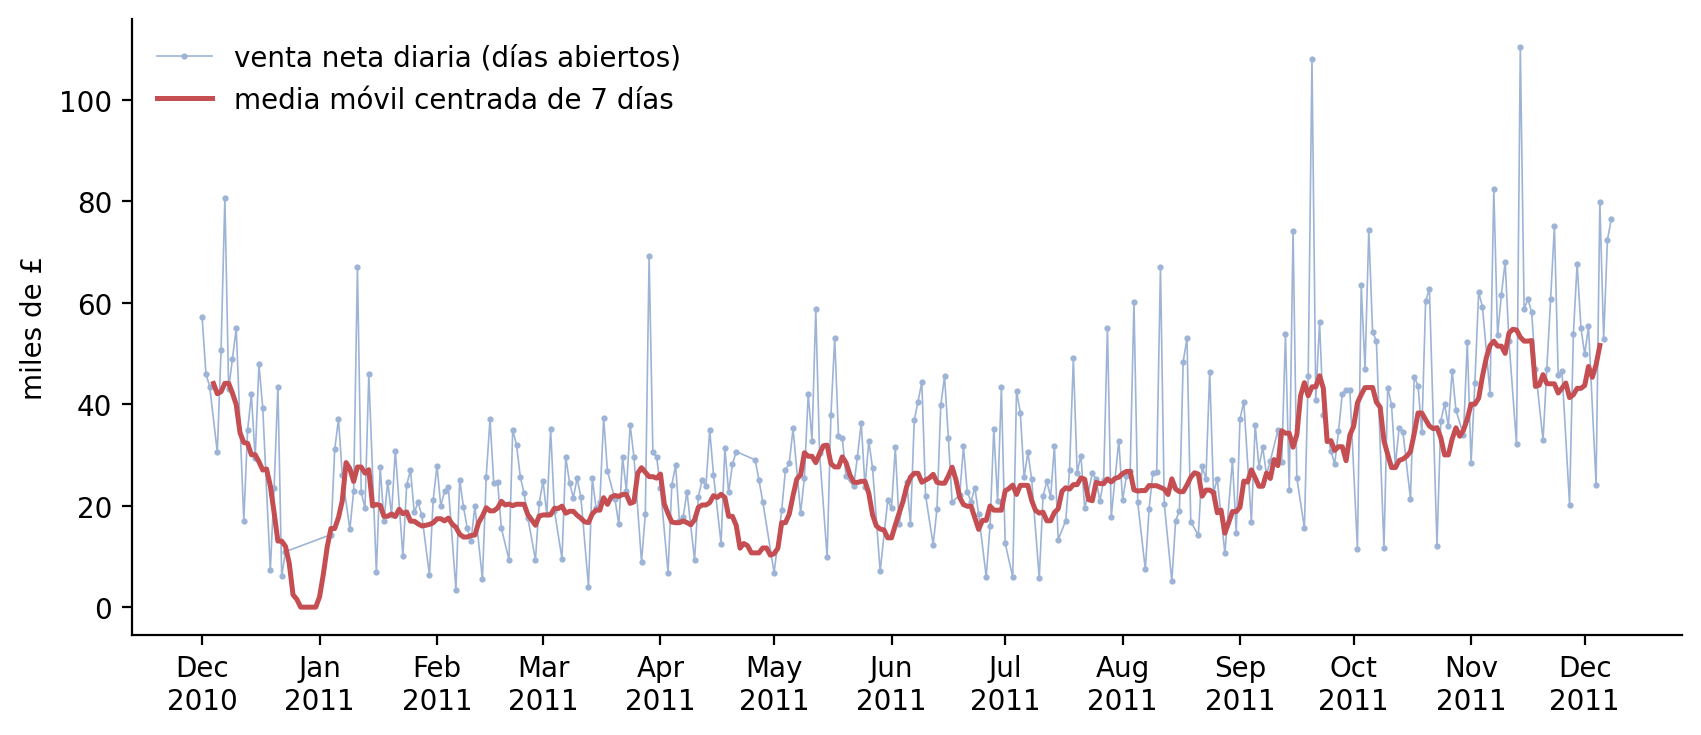
\includegraphics[width=\textwidth]{p3_media_movil.png}
  \caption{Venta neta diaria (días abiertos) y media móvil centrada de 7 días
  calculada con los días cerrados en cero.}
  \label{fig:p3_ma}
\end{figure}

\paragraph{¿Por qué 7?} Porque es el periodo del patrón semanal. Una ventana
de 7 días consecutivos contiene exactamente un lunes, un martes, \dots{} y un
sábado, así que en cada promedio entra cada día de la semana una sola vez y el
patrón semanal se cancela: lo que queda es el nivel de esa semana. Con una
ventana de 5 días la mezcla cambiaría de un día al siguiente (algunas ventanas
tendrían el sábado en cero y otras no, o dos días fuertes y ninguno débil), y
la ``tendencia'' oscilaría con periodo semanal. Con 30 días el patrón semanal
tampoco se cancela exactamente, porque 30 no es múltiplo de 7 (cada ventana
incluye dos días de la semana una vez de más), y además la ventana es tan
ancha que aplana cambios reales de nivel, como el arranque de la temporada en
septiembre o el cierre de Navidad.

\paragraph{¿Por qué centrada?} Para que $MA_t$ describa el nivel
\emph{alrededor} del día $t$, no el de los días anteriores. Una media móvil
de los últimos 7 días (de $t-6$ a $t$) mide el nivel de hace tres días y, en
una serie que sube, siempre se queda atrás. La centrada no tiene ese retraso,
y por eso sirve para descomponer y para dividir $y_t/MA_t$ en el inciso 3.2.
El costo es que usa tres días del futuro, $y_{t+1}$, $y_{t+2}$ y $y_{t+3}$:
sirve para describir la serie, no para pronosticarla. Esto vuelve a aparecer
en el inciso 5.4.

\paragraph{La tendencia.} La venta arranca en diciembre de 2010 alrededor de
\pounds40 mil diarios, se desploma a cero con el cierre de Navidad y en enero
reaparece en un nivel mucho menor. De enero a agosto queda prácticamente
plana: el promedio mensual de la media móvil se mueve entre \pounds17 y
\pounds24 mil, con altibajos de una o dos semanas pero sin dirección clara.
Desde septiembre sube con fuerza, a \pounds32 mil en septiembre, \pounds35
mil en octubre y \pounds47 mil en noviembre y diciembre, más del doble que en
la primera mitad del año. Más que una tendencia lineal es la temporada
navideña de una tienda de regalos que le vende a mayoristas: el nivel de
diciembre de 2011 se parece al de diciembre de 2010.

\subsection{Inciso 3.2: estacionalidad}

Para cada día abierto del entrenamiento se calcula el cociente $y_t/MA_t$, y
el índice estacional de cada día de la semana es el promedio de sus cocientes
(tabla~\ref{tab:p3_indices} y figura~\ref{fig:p3_indices}).

\begin{table}[H]
  \centering
  \small
  \tabla{p3_indices}
  \caption{Índices estacionales con los días abiertos del entrenamiento (1 de
  diciembre de 2010 al 30 de septiembre de 2011). ``Días'' es cuántos
  cocientes entran en cada promedio.}
  \label{tab:p3_indices}
\end{table}

\begin{figure}[H]
  \centering
  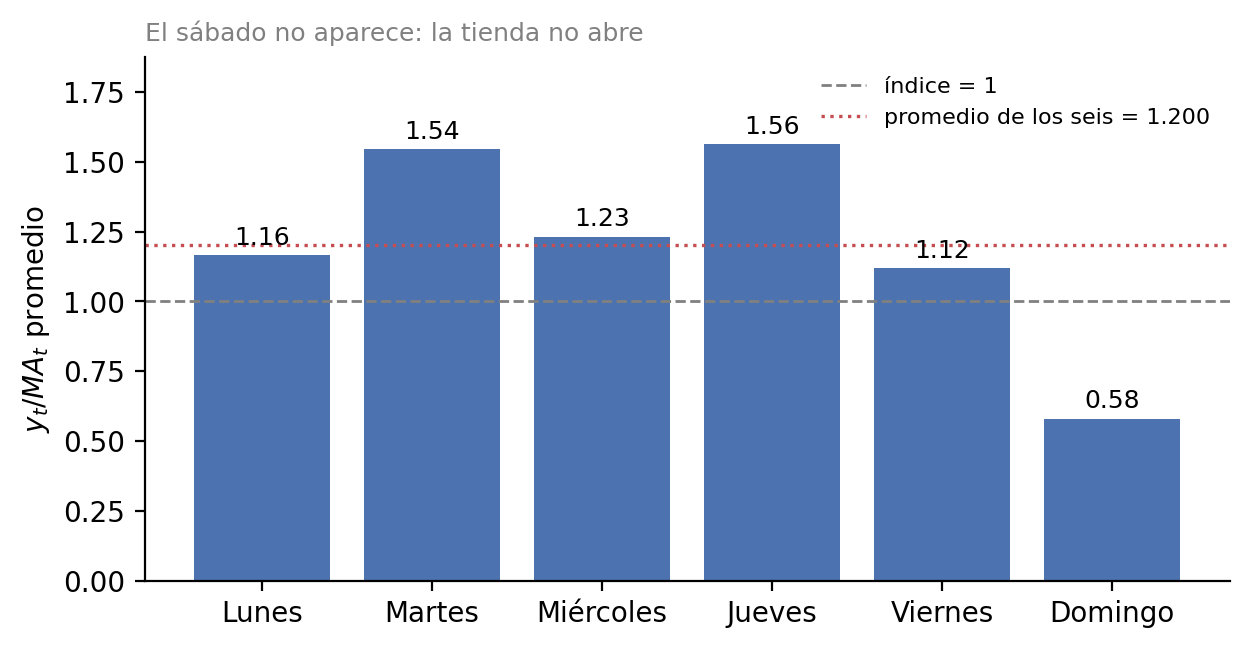
\includegraphics[width=0.75\textwidth]{p3_indices.png}
  \caption{Índice estacional por día de la semana.}
  \label{fig:p3_indices}
\end{figure}

\paragraph{¿Qué días venden más?} Martes (1.54) y jueves (1.56): esos días la
tienda vende en promedio un 55\% más que el nivel de su semana. Les siguen
miércoles (1.23), lunes (1.16) y viernes (1.12). El domingo es claramente el
día débil (0.58). Los cocientes son muy dispersos (desviaciones estándar de
0.3 a 0.5), y los mayores son martes y jueves con pedidos grandes, como el
martes 20 de septiembre, que vendió \pounds108 mil, 2.5 veces la media móvil.
Aun así, el orden no depende de esos extremos: con la mediana en lugar del
promedio, martes y jueves siguen arriba (1.44 y 1.47) y el domingo abajo
(0.53).

\paragraph{¿Por qué el promedio de los seis índices no es 1?} Porque el
séptimo día, el sábado, entra en la media móvil con un cero. Si la venta de
una semana es $V$, la media móvil vale aproximadamente $V/7$, pero esas $V$
libras se reparten entre solo seis días abiertos, que en promedio venden
$V/6$. El cociente promedio de los días abiertos es entonces
$(V/6)/(V/7) = 7/6\approx1.167$. En una descomposición clásica los siete
índices deben promediar 1, y aquí lo hacen si se cuenta el sábado con índice
cero: $(6\times1.2 + 0)/7 \approx 1.03$. El 1.200 observado queda un poco por
encima de 7/6 por dos razones: las semanas con feriado tienen todavía más
ceros en la ventana, lo que baja la media móvil y sube los cocientes de los
días vecinos (el mayor cociente del año es el martes 21 de diciembre de 2010,
justo antes del cierre de Navidad, con 3.33), y el promedio de cocientes no es
el cociente de promedios.

\subsection{Inciso 3.3: autocorrelación}

\paragraph{(a)} Se calcula $r_k$ con la función \texttt{acf} de
\texttt{series.py}, la misma de la Parte 0, sobre los 245 días abiertos del
entrenamiento puestos uno tras otro, una fila por día y sin calendario. Las
bandas son $\pm1.96/\sqrt{245}=\pm0.125$.

\begin{figure}[H]
  \centering
  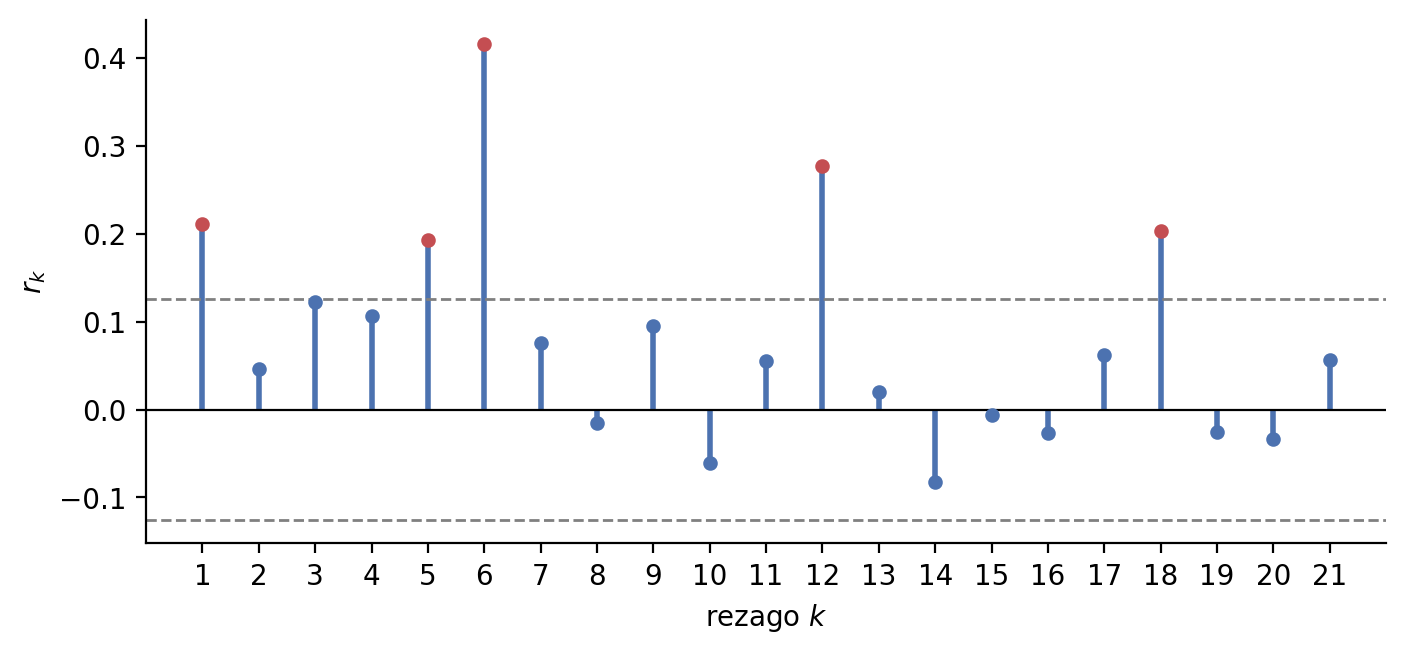
\includegraphics[width=0.85\textwidth]{p3_acf.png}
  \caption{ACF de la venta neta en los días abiertos del entrenamiento
  ($n=245$). En rojo, los rezagos fuera de las bandas.}
  \label{fig:p3_acf}
\end{figure}

\begin{table}[H]
  \centering
  \small
  \tabla{p3_acf}
  \hspace{1.5em}
  \tabla{p3_ljungbox}
  \caption{Izquierda: $r_k$ para $k=1,\dots,21$. Derecha: Ljung--Box sobre la
  serie.}
  \label{tab:p3_acf}
\end{table}

\begin{itemize}
  \item \textbf{Cinco rezagos se salen de las bandas}: 1, 5, 6, 12 y 18. Con
    21 pruebas al 5\% se esperaría uno por azar, no cinco, y menos con el
    patrón que forman.
  \item \textbf{No pasa la prueba de retardo 1} de la Tarea~2:
    $r_1=0.210>0.125$.
  \item \textbf{El pico está en $k=6$}, con $r_6=0.416$, y se repite en sus
    múltiplos: $r_{12}=0.277$ y $r_{18}=0.203$. Como la serie no tiene
    sábados, seis días abiertos hacia atrás son siete días calendario: una
    semana. De los 239 pares de días a distancia 6 en el entrenamiento, 211
    están separados exactamente por 7 días calendario; el resto están más
    separados porque entre ellos hay un feriado o el cierre de Navidad. El
    pico en 6 es el patrón semanal que encontró el inciso 3.2: un martes se
    parece al martes anterior.
  \item \textbf{Ljung--Box lo confirma}: $Q(6)=71.4$ y $Q(12)=96.9$, con
    valores-$p$ del orden de $10^{-13}$ y $10^{-15}$. La serie no es ruido
    blanco por ningún criterio.
\end{itemize}

\paragraph{(b) ¿Memoria o media no constante?} La Parte 0 enseñó a reconocer
las dos huellas. La serie tiene las dos.
\begin{itemize}
  \item Los picos en 6, 12 y 18 son la huella del proceso semanal del inciso
    0.4(b): un patrón que se repite cada semana produce autocorrelación en el
    periodo y sus múltiplos aunque no haya memoria. Es media no constante.
  \item Que casi todos los rezagos de 1 a 9 sean positivos, y que la ACF baje
    despacio, es la huella de la tendencia del inciso 0.4(a): desde septiembre
    todos los días quedan por encima de $\bar y$ y sus vecinos también. Eso
    también es media no constante.
  \item El $r_1=0.21$ puede venir de las dos cosas: de la tendencia o de
    memoria verdadera (un día de ventas altas seguido de otro igual porque los
    clientes compran en rachas). En el proceso semanal de la Parte 0 el patrón
    semanal por sí solo daba un $r_1$ ligeramente \emph{negativo}, así que el
    $r_1$ positivo no lo explica el patrón semanal.
\end{itemize}
Con solo la ACF no se puede separar cuánto es cada cosa. La receta es la del
enunciado: quitar primero la media no constante (el día de la semana, en el
inciso 4.1) y ver qué memoria le queda al residuo.

\section{Parte 4: del AR(1) al SARIMA}
\label{sec:parte4}

Se sigue la receta del enunciado: quitar la estacionalidad, mirar el residuo
y modelar la memoria que quede. Toda la parte usa los 245 días abiertos del
entrenamiento como una fila por día. El código está en \texttt{parte4.py} y la
configuración de S1 y S2 en \texttt{modelos.py}, que se reusa en la Parte~5.

\subsection{Inciso 4.1: quitar el día de la semana}

Se ajusta por OLS $y_t = \sum_{d} \beta_d D_{d,t} + e_t$, con una indicadora
$D_{d,t}$ por cada uno de los seis días abiertos y sin intercepto. Con esa
especificación, cada $\hat\beta_d$ es simplemente la venta promedio de ese día
de la semana: lunes \pounds26\,916, martes \pounds34\,988, miércoles
\pounds27\,695, jueves \pounds35\,266, viernes \pounds26\,208 y domingo
\pounds13\,706. El mismo orden que los índices estacionales del inciso 3.2.

\begin{figure}[H]
  \centering
  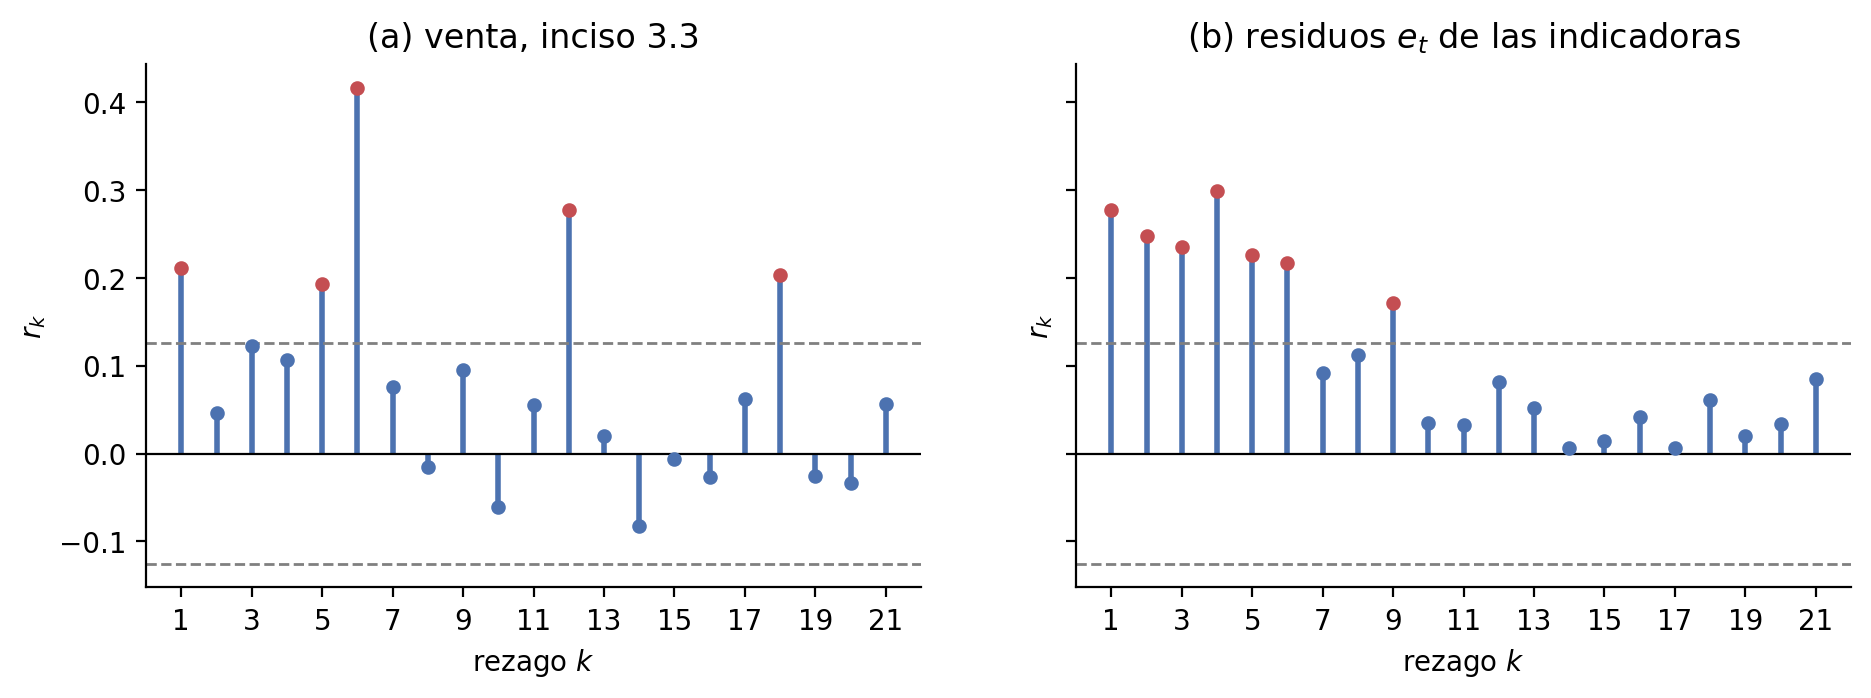
\includegraphics[width=\textwidth]{p4_acf_indicadoras.png}
  \caption{ACF antes (a) y después (b) de quitar el efecto del día de la
  semana, con las mismas bandas $\pm1.96/\sqrt{245}$.}
  \label{fig:p4_acf_ind}
\end{figure}

\paragraph{¿Qué cambió respecto a 3.3?} Los picos en 6, 12 y 18
desaparecieron: $r_{12}$ y $r_{18}$ de los residuos ya están dentro de las
bandas, y $r_6$ bajó de 0.42 a 0.22, al nivel de los rezagos vecinos
(figura~\ref{fig:p4_acf_ind}). Las indicadoras se llevaron el patrón semanal,
que era media no constante, tal como se había anticipado en 3.3(b). Pero lo
que queda no es ruido blanco: los nueve primeros rezagos son positivos y
están fuera de las bandas (salvo el 7 y el 8, que quedan cerca), entre 0.17 y
0.30, y la ACF baja lentamente hasta desaparecer después del rezago 10.
Ljung--Box es todavía mayor que antes ($Q(6)=95.2$; tabla~\ref{tab:p4_lb}).

\paragraph{¿Se parece a un AR(1) o al proceso con tendencia?} Un AR(1) con
$\phi\approx0.28$ (el $r_1$ de los residuos) tendría $r_2\approx0.08$ y
$r_4\approx0.006$: una caída geométrica rápida. Aquí $r_2=0.25$, $r_3=0.24$ y
$r_4=0.30$; la ACF casi no decae en los primeros seis rezagos. Esa es la forma
de la ACF del proceso con tendencia de la Parte 0 (tabla~\ref{tab:p0_sin_memoria}),
donde $r_1$, $r_5$ y $r_7$ eran todos parecidos. El residuo de la
figura~\ref{fig:p4_res} muestra por qué: es positivo casi todo diciembre de
2010 y septiembre de 2011, y negativo casi todo de enero a abril. Los días
vecinos comparten el signo porque comparten el nivel.

\begin{figure}[H]
  \centering
  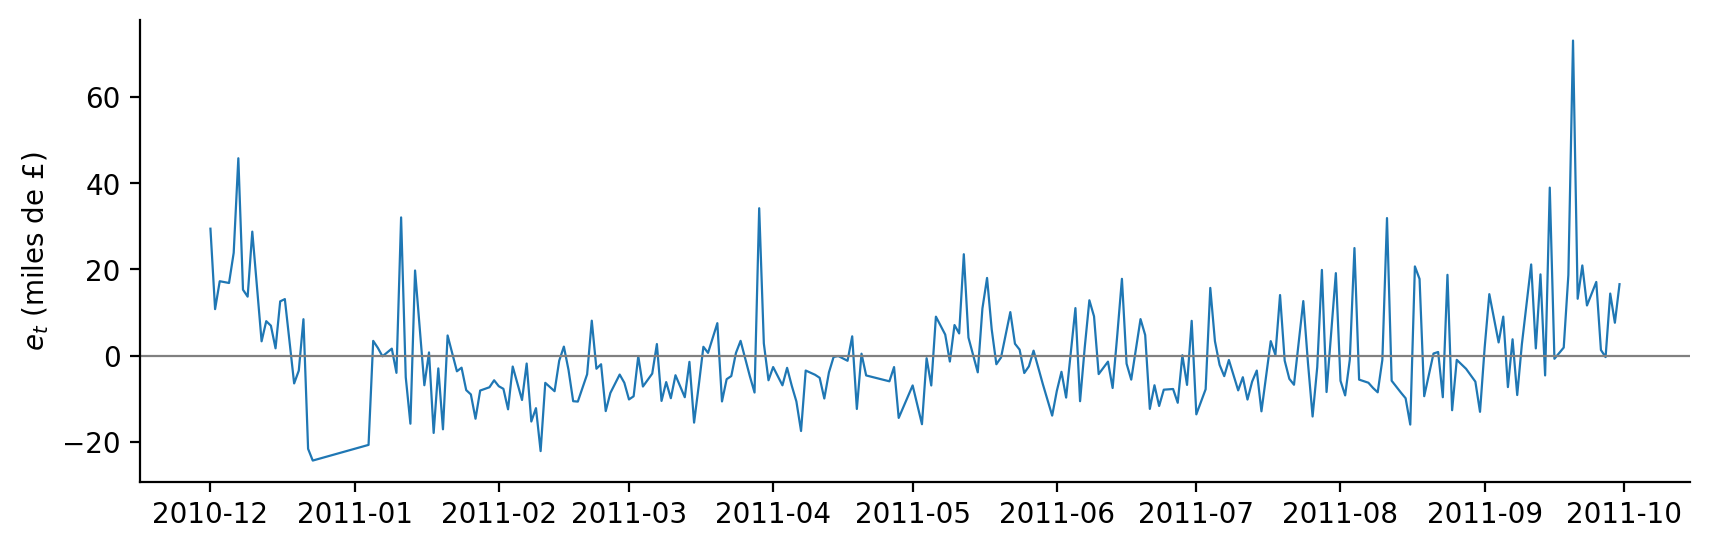
\includegraphics[width=\textwidth]{p4_residuos_indicadoras.png}
  \caption{Residuos $e_t$ de la regresión contra las indicadoras de día de la
  semana.}
  \label{fig:p4_res}
\end{figure}

\paragraph{¿Qué le falta al modelo?} Le falta el nivel. Las indicadoras
suponen que un martes de febrero y un martes de septiembre tienen la misma
media, pero la serie cambia de nivel (inciso 3.1): baja en enero, queda plana
y sube desde septiembre. Ese nivel que se mueve es media no constante que el
modelo no tiene, y queda en los residuos como autocorrelación positiva en
todos los rezagos cortos.

\subsection{Inciso 4.2: un AR(1) sobre los residuos}

Se ajusta por OLS $e_t = c + \phi e_{t-1} + u_t$ y se obtiene
$\hat\phi=0.279$ (con $\hat c=-101.7$, prácticamente cero, como corresponde a
residuos de media cero). La figura~\ref{fig:p4_acf_ar1} es la ACF de
$u_t=e_t-\hat c-\hat\phi e_{t-1}$.

\begin{figure}[H]
  \centering
  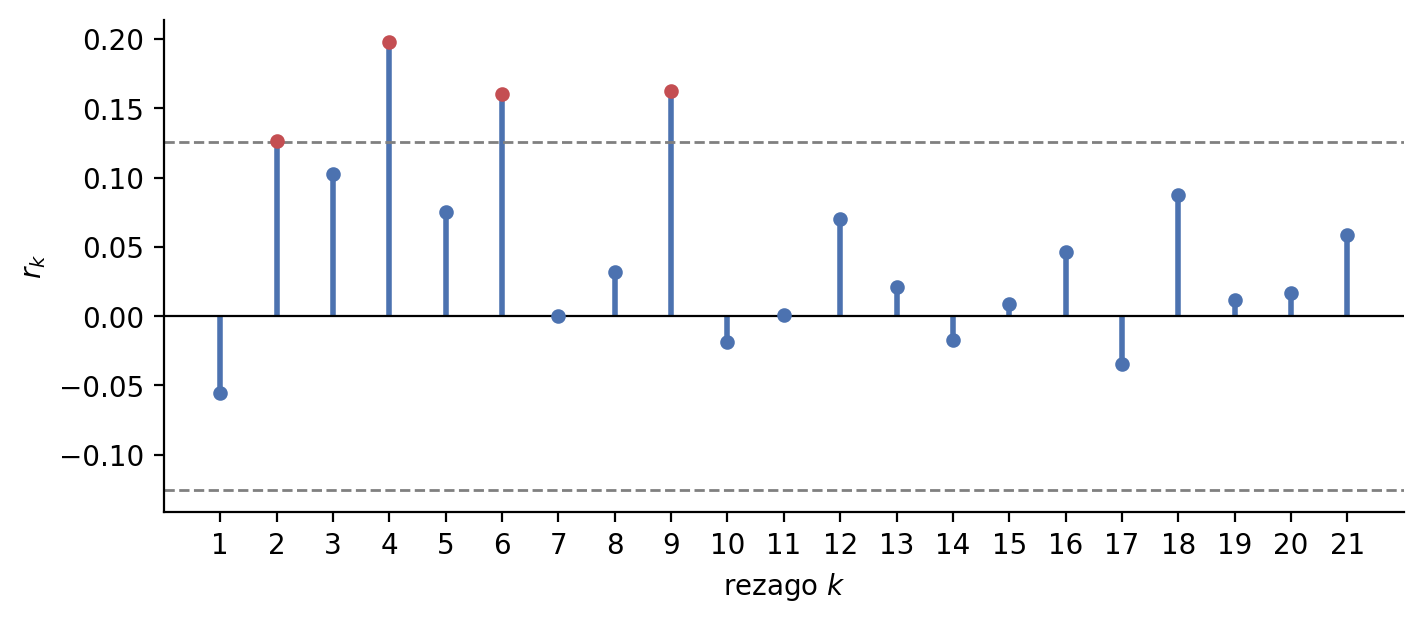
\includegraphics[width=0.8\textwidth]{p4_acf_ar1.png}
  \caption{ACF de los residuos $u_t$ del AR(1) ajustado a $e_t$.}
  \label{fig:p4_acf_ar1}
\end{figure}

\begin{table}[H]
  \centering
  \small
  \tabla{p4_ljungbox}
  \caption{Ljung--Box sobre los residuos de cada etapa. Los grados de
  libertad restan los parámetros de memoria estimados: uno para el AR(1) y
  dos para S1 y S2.}
  \label{tab:p4_lb}
\end{table}

Todavía no son ruido blanco. El AR(1) se llevó el rezago 1 ($r_1$ pasó de
0.28 a $-0.06$), pero siguen fuera de las bandas los rezagos 2, 4, 6 y 9
($r_4=0.20$, $r_6=0.16$, $r_9=0.16$). Ljung--Box lo confirma: $Q(6)=25.1$ con 5
grados de libertad y $Q(12)=33.4$ con 11, con valores-$p$ de $10^{-4}$. Un
AR(1) no alcanzó, y era de esperarse: el AR(1) modela una memoria que se
desvanece geométricamente, y lo que había en 4.1 era un nivel que se mueve
durante meses. El AR(1) solo puede representarlo como ``hoy se parece a
ayer'', y por eso arregla el rezago 1 y deja el resto.

\subsection{Inciso 4.3: SARIMA}

Con \texttt{statsmodels.tsa.statespace.sarimax.SARIMAX} se ajustan, sobre
$\log y_t$, los dos modelos con $s=6$:
\begin{align*}
  \text{S1:}\quad & (1-\phi B)(1-\Phi B^6)(\log y_t - \mu) = \varepsilon_t,
    \qquad\text{SARIMA}(1,0,0)(1,0,0)_6 \text{ con constante;}\\
  \text{S2:}\quad & (1-B)(1-B^6)\log y_t = (1+\theta B)(1+\Theta B^6)\varepsilon_t,
    \qquad\text{SARIMA}(0,1,1)(0,1,1)_6 \text{ sin constante.}
\end{align*}
A \texttt{SARIMAX} se le pasa el arreglo de valores, no la serie con fechas.
En \texttt{statsmodels} la constante de S1 se estima como el intercepto $c$
de la ecuación, que se relaciona con la media por
$c=\mu(1-\phi)(1-\Phi)$.

\paragraph{¿Por qué $s=6$ y no 7?} Porque el modelo trabaja con una fila por
día abierto, y una semana tiene seis días abiertos: el martes anterior está
seis filas atrás, no siete (el pico de la ACF del inciso 3.3 estaba en 6). Con
$s=7$ el modelo compararía cada día con un día de la semana distinto cada vez.

\paragraph{¿Cuándo se rompe esa suposición?} Cuando una semana tiene menos de
seis días abiertos. Después de un feriado, seis filas atrás ya no es el mismo
día de la semana: después del Lunes de Pascua (25 de abril), por ejemplo, las
filas quedan desfasadas un día durante una semana, y el modelo compara un
martes con un miércoles. El caso extremo es el cierre de Navidad, que se come
nueve días. Según el inciso 3.3, 28 de los 239 pares de días a distancia 6 no
están a una semana; en esos puntos la estacionalidad del modelo apunta al día
equivocado.

\paragraph{¿Por qué el logaritmo?} Porque la variación de la serie crece con
su nivel. En febrero la venta diaria promedia \pounds20.7 mil con una
desviación estándar de \pounds8.5 mil; en septiembre promedia \pounds38.9 mil
y la desviación sube a \pounds18.9 mil. En logaritmo, la desviación estándar
mensual queda entre 0.35 y 0.69 durante todo el año, sin crecer con el
nivel. Además, los índices
estacionales del inciso 3.2 son multiplicativos: el martes vende un 55\% más
que su semana, no una cantidad fija de libras más. FPP2 (§3.2) recomienda
transformar cuando la variación depende del nivel. El logaritmo convierte la
estructura multiplicativa en aditiva, $\log y_t = \log T_t + \log S_t + \log
R_t$, que es lo que un SARIMA sabe modelar, y estabiliza la varianza. Además
garantiza que el pronóstico en libras, $\exp(\cdot)$, sea positivo. Se puede
usar porque en los días abiertos la venta neta es siempre positiva: el mínimo
del entrenamiento es \pounds3\,440.

\paragraph{Convergencia.} La tabla~\ref{tab:p4_sarima} muestra los
parámetros con el límite de iteraciones por defecto (50) y con 500.

\begin{table}[H]
  \centering
  \small
  \tabla{p4_sarima}
  \caption{Parámetros de S1 y S2 sobre $\log y_t$ con 50 y 500 iteraciones
  como máximo. ``Convergió'' es \texttt{mle\_retvals['converged']}.}
  \label{tab:p4_sarima}
\end{table}

S2 converge en 14 iteraciones y sus parámetros no cambian al subir
\texttt{maxiter}. S1 \emph{no} converge con el valor por defecto: se detiene en
la iteración 50 con $\Phi=0.906$, $\phi=0.164$ y $c=0.795$. Con
\texttt{maxiter=500} converge en 81 iteraciones a un modelo distinto:
$\Phi=0.521$, $\phi=0.132$ y $c=4.210$, con una log-verosimilitud mucho
mayor ($-160.7$ contra $-185.9$). Lo interesante es que los dos conjuntos de
parámetros implican casi la misma media, $\mu=c/((1-\phi)(1-\Phi))\approx
10.12$ en logaritmo, es decir, \pounds24\,900 diarios. Lo que cambia es la
dinámica: el optimizador sin terminar estaba en una región con $\Phi$ cerca
de 1, casi una raíz unitaria estacional, que es un modelo con mucha más
memoria semanal de la que tienen los datos. Sin revisar
\texttt{mle\_retvals} se habría usado ese modelo sin saberlo. De aquí en
adelante S1 se ajusta siempre con \texttt{maxiter=500}.

\subsection{Inciso 4.4: diagnóstico}

Los residuos de S2 empiezan con valores enormes ($10.9$ en el primero y
$-6.1$ en el séptimo, cuando los demás son del orden de $\pm0.5$): con
inicialización difusa, las primeras $1+6=7$ observaciones solo sirven para
arrancar las diferencias $(1-B)(1-B^6)$ y sus residuos no significan nada. Se
descartan. La figura~\ref{fig:p4_acf_sarima} y la tabla~\ref{tab:p4_lb}
muestran el resultado, con $m-2$ grados de libertad.

\begin{figure}[H]
  \centering
  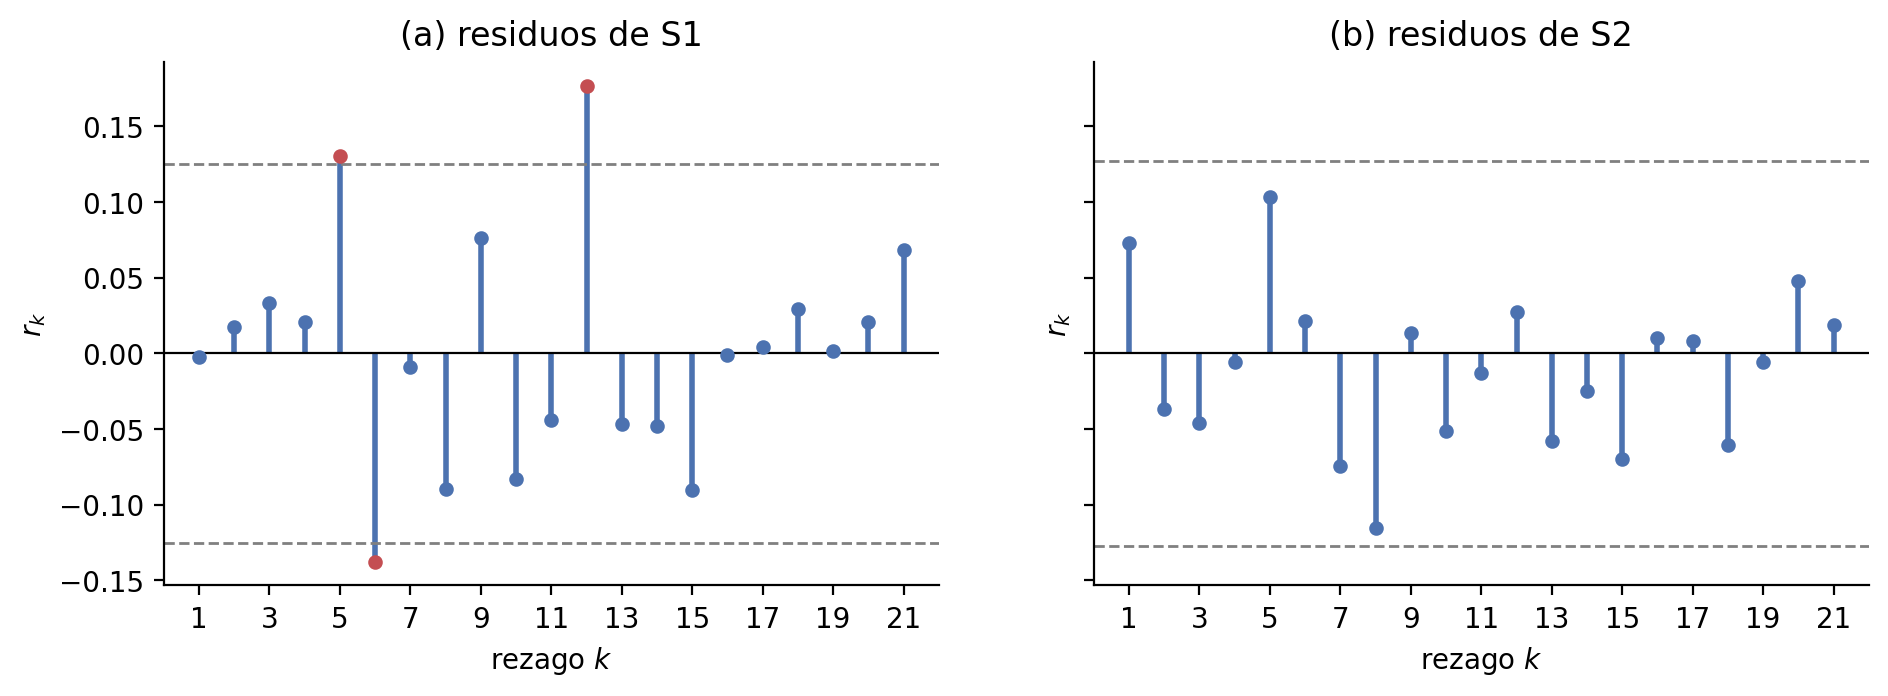
\includegraphics[width=\textwidth]{p4_acf_sarima.png}
  \caption{ACF de los residuos de S1 (con \texttt{maxiter=500}) y de S2 (sin
  sus primeros 7 residuos).}
  \label{fig:p4_acf_sarima}
\end{figure}

\begin{itemize}
  \item \textbf{S1 no deja ruido blanco.} $Q(6)=9.5$ con 4 grados de
    libertad ($p=0.049$, justo en la frontera) y $Q(12)=23.5$ con 10
    ($p=0.009$): se rechaza ruido blanco. S1 modela la memoria y el patrón
    semanal, pero alrededor de una media \emph{fija}, y el cambio de nivel que
    se vio en 4.1 sigue en sus residuos.
  \item \textbf{S2 sí.} $Q(6)=4.9$ ($p=0.30$) y $Q(12)=10.5$ ($p=0.40$):
    no hay evidencia de autocorrelación en sus residuos. La diferencia
    $(1-B)$ es lo que le permite seguir un nivel que se mueve, y $(1-B^6)$
    se lleva el patrón semanal.
\end{itemize}

\subsection{Inciso 4.5: hacia dónde van los pronósticos}

La figura~\ref{fig:p4_horizonte} muestra los pronósticos de los dos modelos,
ajustados con todo el entrenamiento, para los siguientes 120 días abiertos.

\begin{figure}[H]
  \centering
  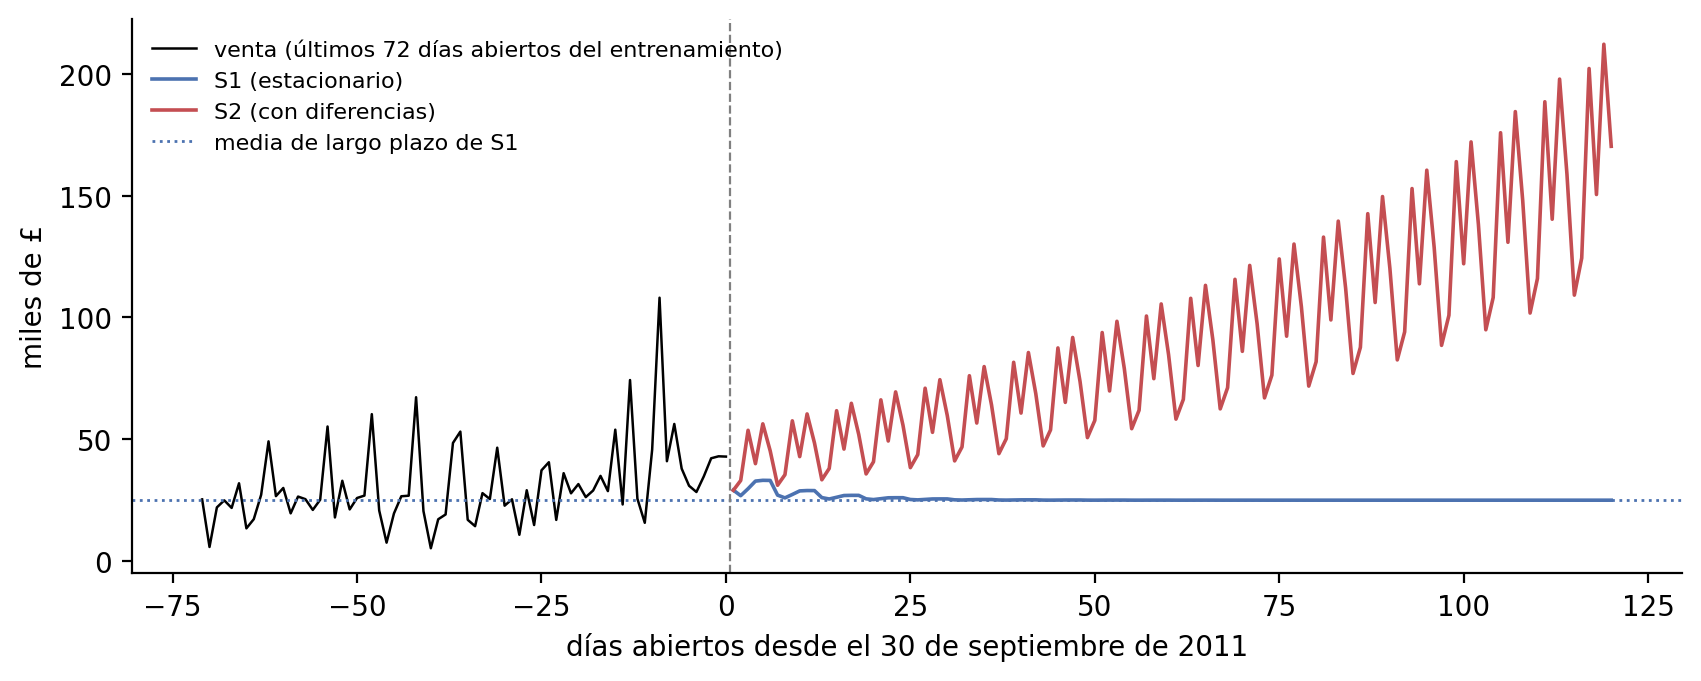
\includegraphics[width=\textwidth]{p4_horizonte.png}
  \caption{Pronósticos de S1 y S2 hasta 120 días abiertos después del 30 de
  septiembre de 2011, en libras ($\exp$ del pronóstico en logaritmo).}
  \label{fig:p4_horizonte}
\end{figure}

\paragraph{S1 regresa a su media.} Es estacionario, y en un AR estacionario el
efecto de lo observado decae como $\phi^h$ (inciso 0.1). Para S1 las dos
memorias, $\phi^h$ con $\phi=0.13$ y $\Phi^{h/6}$ con $\Phi=0.52$, se
desvanecen en unas pocas semanas, y el pronóstico converge a
$\exp(\mu)\approx$ \pounds24\,875 diarios, la venta típica de enero a
septiembre. A partir de un mes de horizonte, S1 pronostica lo mismo para
todos los días: ni siquiera conserva el patrón semanal, porque ese patrón
también lo modelaba como memoria que se desvanece.

\paragraph{S2 no regresa a ningún lado.} Igual que la caminata aleatoria, que
nunca olvida, S2 no tiene una media a la cual volver: su pronóstico arranca
del último nivel observado y conserva el último patrón semanal. Y como tiene
dos diferencias ($d=1$ y $D=1$), el pronóstico admite además una pendiente: la
estima con el promedio reciente de los cambios, y el crecimiento de septiembre
la hace positiva, así que la proyecta sin límite. A 120 días abiertos el
pronóstico supera las \pounds200 mil diarias. A horizontes cortos, ese
comportamiento es justo lo que S1 no puede hacer (seguir un nivel nuevo); a
horizontes largos, una extrapolación así es peligrosa. Para un pronóstico de
una semana, que es lo que pide la Parte 5, lo que importa es el corto plazo.

% \section{Parte 5: pronóstico y fuga}
\label{sec:parte5}

Cada modelo está implementado en \texttt{parte5.py} como una función que
recibe la serie, el origen (un domingo) y los días abiertos de la semana
siguiente, y que solo puede mirar la serie hasta el origen. El origen móvil
sigue exactamente las reglas del enunciado: los objetivos son los días
abiertos de lunes a domingo después del origen; en (b) no se evalúa nada
después del 30 de septiembre y en (c) el último día es el 8 de diciembre; para
S1 y S2 el horizonte es la posición del objetivo entre los días abiertos
posteriores al origen; y el MAE y el RMSE juntan todos los días pronosticados.
En (b) hay 22 orígenes, del 1 de mayo al 25 de septiembre, con 128 días
evaluados; en (c) hay 10, del 2 de octubre al 4 de diciembre, con 58.

\subsection{Inciso 5.1: los modelos}

\begin{itemize}
  \item \textbf{B1}: el promedio de todos los días abiertos hasta el origen.
  \item \textbf{B2} (\emph{naive} estacional): para cada objetivo, la venta del
    mismo día de la semana abierto más reciente hasta el origen.
  \item \textbf{M1}: OLS de $y_t$ contra $t$ (días desde el 1 de diciembre de
    2010) y las seis indicadoras de día de la semana.
  \item \textbf{M2}: OLS de $y_t$ contra las seis indicadoras, $y_{t-7}$ y
    $y_{t-14}$. Si el día del rezago está cerrado se usa el mismo día de la
    semana abierto más reciente; el código verifica con un \texttt{assert} el
    ejemplo del enunciado (para el 9 de mayo, $y_{t-7}$ es la venta del 18 de
    abril, \pounds31\,402). Para $y_{t-14}$ se aplica la misma regla, así que
    el 9 de mayo sus dos rezagos son el 18 de abril. Las 12 filas del inicio
    que no tienen rezago no se usan para ajustar.
  \item \textbf{S1} y \textbf{S2}: los modelos del inciso 4.3, reajustados en
    cada origen con todos los días abiertos hasta el origen y llevados a
    libras con $\exp(\cdot)$.
\end{itemize}

\paragraph{¿Por qué M2 puede usar $y_{t-7}$ pero no $y_{t-1}$?} El
pronóstico se hace el domingo para toda la semana siguiente. Para cualquier
objetivo de lunes a domingo, siete días antes cae en el domingo de origen o
antes, así que $y_{t-7}$ ya se observó: el lunes usa el lunes anterior y el
domingo usa el propio domingo de origen. En cambio, $y_{t-1}$ solo se conoce
para el lunes; para el martes, $y_{t-1}$ es el lunes, que el domingo todavía
no ha ocurrido. Una regresión que lo usara como variable necesitaría un dato
del futuro.

\paragraph{¿Cómo usa S1 el rezago 1 de todas formas?} De forma recursiva. Un
modelo autorregresivo pronostica un paso a la vez y, cuando le falta un
valor, usa su propio pronóstico en su lugar: $\hat y_{t+2} = c + \phi\,\hat
y_{t+1} + \dots$. El filtro de Kalman de \texttt{SARIMAX} hace exactamente
eso. Por eso la información del último día observado se diluye como $\phi^h$
conforme crece el horizonte $h$: con $\phi\approx0.13$, para el martes ya casi
no queda nada del domingo. M2 no puede hacer esto porque es una regresión
directa: no pronostica sus propias variables.

\paragraph{Convergencia en cada origen.} Se reajustan S1 y S2 en los 32
orígenes de (b) y (c), con la configuración del inciso 4.3
(\texttt{maxiter=500}), y se revisa \texttt{mle\_retvals['converged']} en
cada uno. S2 convergió en los 32. S1 convergió en 31; en el del 1 de mayo
L-BFGS se detuvo en la iteración 52 con \texttt{warnflag=2}, que significa que
la búsqueda de línea ya no lograba mejorar. No fue por falta de iteraciones:
con 1\,000 o 2\,000 se detiene en el mismo punto, con un gradiente del orden
de $10^{-4}$. El código reintenta con BFGS, que sí converge, a los mismos
parámetros hasta el segundo decimal y con log-verosimilitud $-80.3911$ contra
$-80.3912$. Los pronósticos cambian menos de \pounds12. Es decir, el ajuste
estaba en el óptimo y el optimizador no lo pudo certificar; aun así se usa el
ajuste que sí convergió.

\subsection{Inciso 5.2: tres formas de estimar el error}

La tabla~\ref{tab:p5_errores} reúne los tres esquemas. En (a), cada celda es
la media $\pm$ la desviación estándar sobre las 10 semillas
(\texttt{SEMILLAS\_CV} en \texttt{semillas.py}) de una validación cruzada
aleatoria de 5 \emph{folds} sobre los días abiertos del entrenamiento.

\begin{table}[H]
  \centering
  \small
  \tabla{p5_errores}
  \caption{MAE y RMSE en libras: (a) validación cruzada aleatoria de 5
  \emph{folds} en el entrenamiento, con 10 semillas; (b) origen móvil semanal
  en el entrenamiento, orígenes de mayo a septiembre; (c) origen móvil
  semanal en la prueba.}
  \label{tab:p5_errores}
\end{table}

\paragraph{¿Por qué no tiene sentido (a) para B2, S1 y S2?} Porque los tres
dependen del orden de la serie, y la validación cruzada aleatoria lo destruye.
Al sacar al azar un 20\% de los días, el día a pronosticar queda rodeado de
días de entrenamiento \emph{posteriores} a él. Para B2, ``el mismo día de la
semana más reciente'' de un día de marzo podría ser un día de abril, y eso ya
no es un pronóstico sino una interpolación. S1 y S2 necesitan la secuencia
completa para que $B$ y $B^6$ signifiquen ``ayer'' y ``hace una semana'': con
huecos aleatorios el rezago $k$ deja de ser un rezago fijo, y el filtro, al
estimar un día faltante, usaría los días siguientes. B1, M1 y M2 son
regresiones cuyas filas se pueden repartir entre \emph{folds}, así que
mecánicamente sí se puede calcular (a) para ellas. Pero también están
contaminadas: M1 estima la pendiente con días posteriores al que pronostica, y
el nivel de los días vecinos (que son los que más se parecen) siempre queda
en el entrenamiento.

\paragraph{¿Cuál se acerca más a (c)?} El origen móvil. Para M1 y M2, (b)
da errores más grandes que (a) y, por lo tanto, más cercanos a (c): M2 pasa
de 8\,345 en (a) a 9\,258 en (b), contra 15\,219 en (c), y M1 de 9\,129 a
9\,833, contra 15\,203. Para B1 los dos esquemas coinciden (10\,271 y
10\,253): la media histórica no tiene cómo aprovechar a los vecinos de un
día, así que la validación aleatoria no le regala nada. La validación cruzada aleatoria es
la más optimista porque es la que más información del futuro deja entrar.

\paragraph{¿Alguna se acerca de verdad?} No. El error en la prueba es entre
1.25 y 2.2 veces el de (b), y además el orden de los modelos cambia por
completo. En (b) el mejor es M2 y S2 queda cuarto, por delante solo de B1 y
B2; en (c) S2 es claramente el mejor y M2 queda en el lugar cuatro, empatado
con M1. Ninguna estimación hecha dentro del entrenamiento habría escogido el
modelo ganador. El inciso 5.5 discute por qué.

\subsection{Inciso 5.3: qué modelo gana en la prueba}

\textbf{Gana S2}, con MAE de \pounds12\,545 y RMSE de \pounds15\,901: un 13\%
menos de MAE que el segundo lugar (B2, \pounds14\,409) y un 18\% menos que M1
y M2. La figura~\ref{fig:p5_prueba} muestra los pronósticos de todos los
modelos contra la serie real.

\begin{figure}[H]
  \centering
  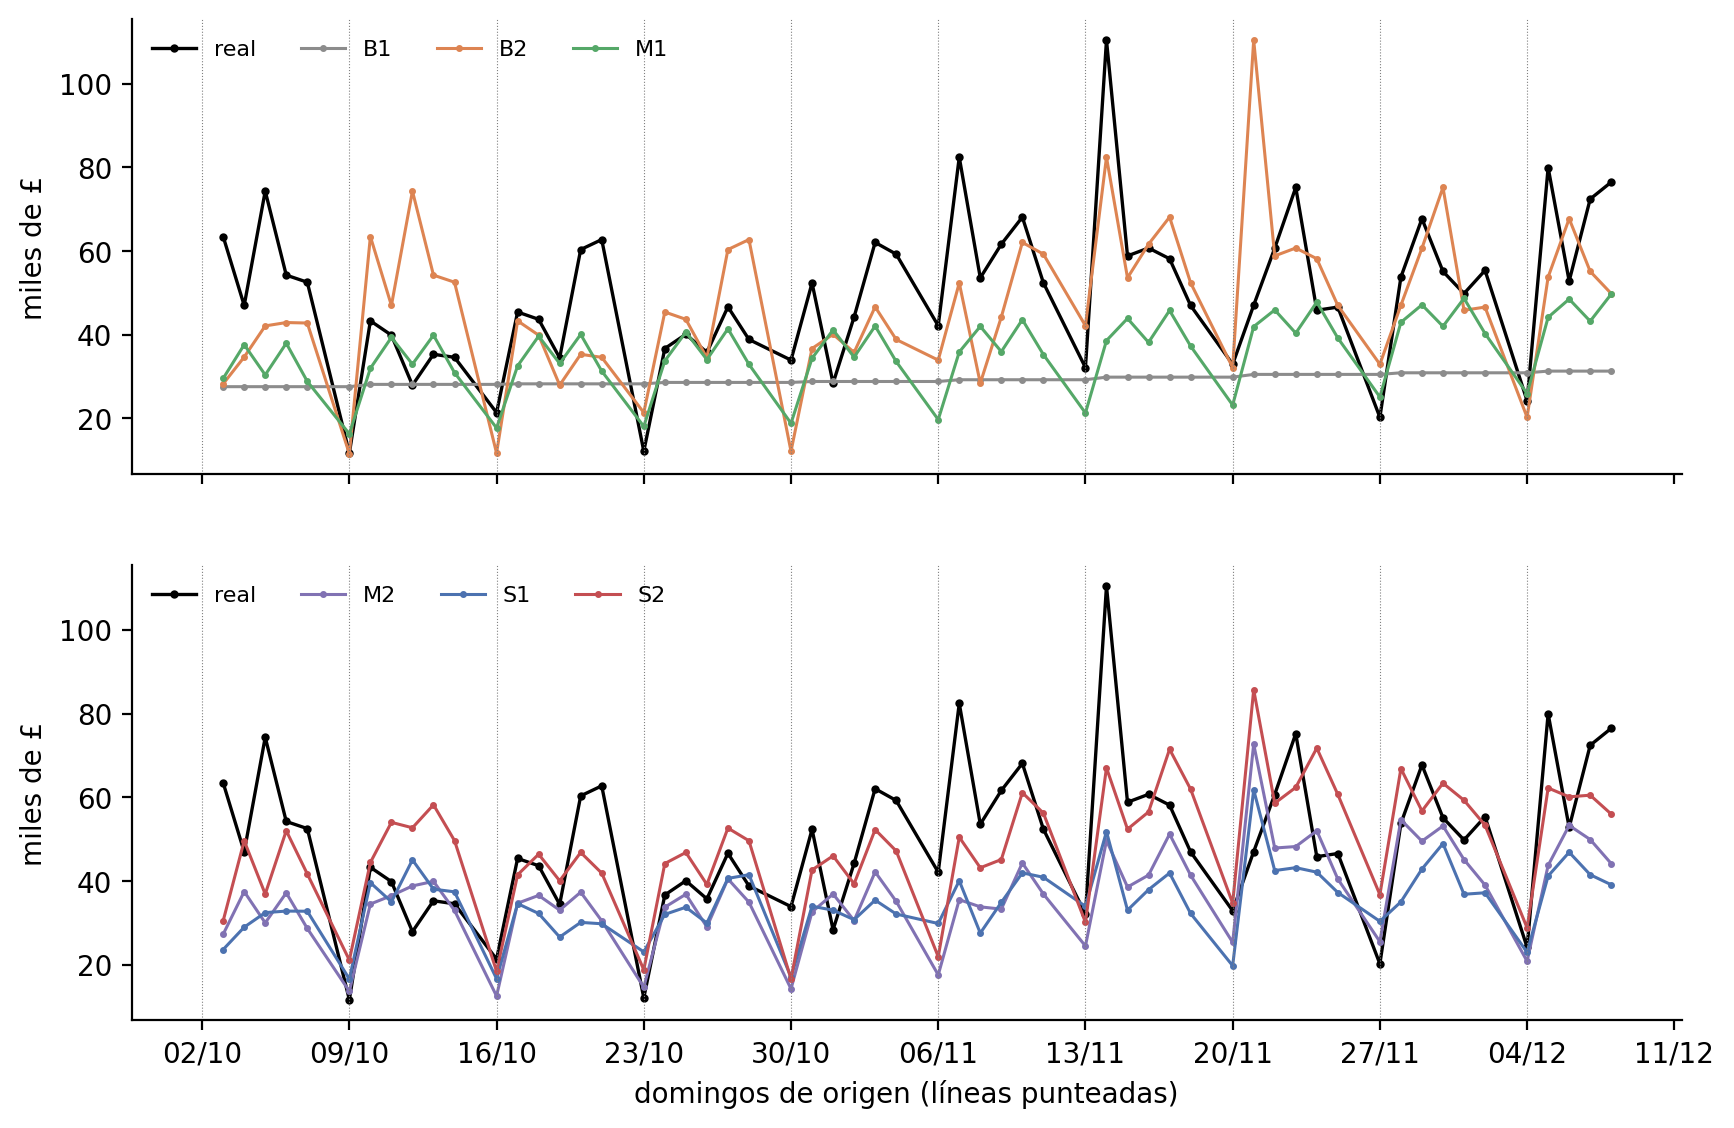
\includegraphics[width=\textwidth]{p5_pronosticos_prueba.png}
  \caption{Pronósticos con origen móvil semanal en la prueba (octubre a
  diciembre de 2011) contra la venta real. Cada línea punteada es un domingo
  de origen; cada modelo pronostica los seis días abiertos que le siguen.}
  \label{fig:p5_prueba}
\end{figure}

\begin{table}[H]
  \centering
  \small
  \tabla{p5_sesgo}
  \caption{Error medio en la prueba (real menos pronóstico), en libras. Un
  valor positivo significa que el modelo se queda corto.}
  \label{tab:p5_sesgo}
\end{table}

\paragraph{Por qué gana S2.} La prueba es la temporada navideña: la venta
media de los días evaluados en (c) es \pounds49\,800, contra \pounds29\,500
en (b). La tabla~\ref{tab:p5_sesgo} muestra qué hace cada modelo con ese
cambio de nivel. B1, M1, M2 y S1 se quedan cortos, en promedio, por
\pounds13\,000 a \pounds20\,500 diarios. B1 promedia todo el año. M1 ajusta
una sola recta a un año que fue plano ocho meses y luego subió, y la recta
queda por debajo del final. M2 le da poco peso a los rezagos (el día de la
semana explica casi todo en el entrenamiento). Y S1, como se vio en el inciso
4.5, regresa a una media estimada con enero a septiembre. En la
figura~\ref{fig:p5_prueba} se ve que sus pronósticos tienen la forma semanal
correcta pero quedan sistemáticamente por debajo de la línea negra a partir
de noviembre.

Solo dos modelos casi no tienen sesgo: B2 (\pounds2\,743) y S2
(\pounds1\,187). Los dos parten de lo que pasó la semana anterior y, por lo
tanto, siguen el nivel. La diferencia entre ellos es el ruido: B2 copia una
sola semana, con todos sus picos, así que cuando el martes anterior tuvo un
pedido excepcional lo repite (para el lunes 21 de noviembre pronostica
\pounds110 mil porque ese fue el pico real del lunes 14; la venta fue de
\pounds47 mil). S2 hace lo mismo pero promediando: sus
términos de promedio móvil, $\theta=-0.91$ y $\Theta=-0.67$, convierten la
diferencia en un promedio exponencialmente ponderado de las semanas
recientes. Sigue el nivel como B2, pero sin copiar el ruido.

Esto es coherente con el diagnóstico del inciso 4.4: S2 fue el único modelo
cuyos residuos parecían ruido blanco, porque fue el único que capturó el
nivel que se mueve. S1 dejaba autocorrelación en los residuos, justamente por
ese nivel, y en la prueba eso se convierte en sesgo. En (b), de mayo a
septiembre, el nivel fue estable y modelos que regresan a la media no pagaban
ese costo; la flexibilidad de S2 solo le añadía varianza. En la prueba, el
nivel se movió y esa flexibilidad es la que gana.

\begin{table}[H]
  \centering
  \small
  \tabla{p5_semanas}
  \caption{MAE de cada semana de la prueba, en miles de libras. ``Mejor'' es
  el modelo con menor MAE esa semana.}
  \label{tab:p5_semanas}
\end{table}

La victoria no es de todas las semanas (tabla~\ref{tab:p5_semanas}): S2 es el
mejor en 5 de las 10 y M1 en 3, siempre en semanas tranquilas, sin cambio de
nivel. Pero S2 nunca tiene una semana desastrosa, y por eso gana en el total.
Los errores más grandes de todos los modelos vienen de días con pedidos
excepcionales, como el lunes 14 de noviembre (\pounds110 mil), que ningún
modelo podía anticipar.

\subsection{Inciso 5.4: la trampa}

Se agrega a M2 la media móvil centrada de 7 días de la Parte 3, calculada una
sola vez sobre toda la serie, como una variable más.

\begin{table}[H]
  \centering
  \small
  \tabla{p5_trampa}
  \caption{M2 con y sin la media móvil centrada como predictor. (a):
  promedio sobre 10 semillas; (b): origen móvil en el entrenamiento.}
  \label{tab:p5_trampa}
\end{table}

\paragraph{Se ve mejor.} Mucho mejor: el MAE baja de 8\,345 a 7\,450 en (a) y
de 9\,258 a 8\,377 en (b), alrededor de un 10\% en los dos esquemas
(tabla~\ref{tab:p5_trampa}). El ajuste con todo el entrenamiento le da a la
media móvil un coeficiente de 1.05 y deja los rezagos en prácticamente cero
(0.01 y 0.05): el modelo descubre que la mejor forma de pronosticar la venta
de un día es ``la media móvil de ese día más el efecto del día de la semana''.

\paragraph{Por qué es ilegal.} Porque $MA_t$ contiene el futuro. La media
centrada del día $t$ promedia de $y_{t-3}$ a $y_{t+3}$, así que incluye la
venta del propio día que se quiere pronosticar ($y_t$, con peso $1/7$) y la
de los tres días siguientes. El domingo de origen, para pronosticar el lunes
se necesitarían las ventas de lunes a jueves; para pronosticar el jueves,
hasta las del domingo siguiente. Ningún dato de la semana objetivo existe
cuando se hace el pronóstico.

\paragraph{Por qué el origen móvil no lo detecta.} Porque el origen móvil solo
controla qué \emph{filas} entran al ajuste; no revisa cómo se calcularon las
\emph{variables} de esas filas. Si la media móvil se calcula una vez sobre toda
la serie y luego se parte en orígenes, la columna \texttt{ma7} del lunes
objetivo ya trae adentro las ventas de la semana objetivo, aunque esas filas
no se hayan usado para estimar los coeficientes. La fuga está en la
construcción de la variable, antes de la validación, y ninguna partición de
filas la puede ver. La única defensa es recalcular cada variable en cada
origen usando solo datos hasta el origen, y con la media centrada eso es
imposible para la semana objetivo.

\paragraph{Por qué (c) no se puede calcular sin hacer trampa.} En la prueba,
para el origen del 2 de octubre la media móvil de los objetivos necesita las
ventas del 3 al 11 de octubre, que son precisamente los valores que se están
evaluando. Calcular (c) con esa variable es darle al modelo parte de la
respuesta del examen. La versión honesta requeriría pronosticar primero la
media móvil, es decir, pronosticar las ventas de la semana, que es justo el
problema que se quería resolver. Por eso esta variable no tiene versión
legítima para pronosticar, y por eso su mejora en (a) y (b) es una ilusión.

\subsection{Inciso 5.5: por qué el entrenamiento se queda corto}

Todas las estimaciones hechas dentro del entrenamiento subestiman el error de
la prueba. Hay dos causas, y conviene separarlas.

\paragraph{1. Cómo se partieron los datos.} La validación cruzada aleatoria
deja que el modelo aprenda del futuro y que el día pronosticado esté rodeado
de días vecinos en el entrenamiento, que comparten su nivel. Es lo que separa
(a) de (b): de 8\,345 a 9\,258 en M2, de 9\,129 a 9\,833 en M1. \emph{Esta
causa sí se arregla con una mejor validación}: el origen móvil reproduce las
condiciones reales del pronóstico (solo pasado, horizonte de una semana) y la
elimina.

\paragraph{2. La serie cambió.} La prueba es la temporada navideña, con una
venta media de \pounds49\,800 contra \pounds29\,500 de los días evaluados en
(b), y los errores crecen con el nivel. Si el MAE se divide entre la venta
media de los días evaluados, los modelos tienen errores relativos parecidos
en los dos periodos: entre 31\% y 38\% en (b), y entre 25\% y 45\% en (c). M2,
por ejemplo, tiene un 31\% en ambos. Lo que más cambia es para quién: B1 y
S1, que regresan a la media, empeoran en términos relativos; S2 y B2, que
siguen el nivel, mejoran. \emph{Esta causa no se arregla con ninguna
validación}: no existe forma de que una validación dentro de enero a
septiembre mida cómo se comporta un modelo en un régimen que el entrenamiento
nunca contuvo. Lo único que ayuda es tener datos de ese régimen, o un modelo
que se adapte a cambios de nivel (como S2), y aun así sin poder medir de
antemano cuánto.

\paragraph{¿Se puede estimar la estacionalidad anual con un año de datos?}
No. Para estimar un patrón que se repite cada año hay que verlo repetirse,
es decir, al menos dos años completos; FPP2 lo plantea igual para cualquier
estacionalidad. Con un año, cada día del año aparece una sola vez, y el
``efecto noviembre'' es indistinguible de una tendencia, de un cambio en la
clientela o de un evento único: los tres producen la misma subida desde
septiembre. Además, el único otro diciembre de los datos (el de 2010) está
partido por el cierre de Navidad. Es justamente lo que le faltó a todos los
modelos: ninguno sabía que el cuarto trimestre vende el doble, porque en el
entrenamiento no había un cuarto trimestre del cual aprenderlo.

% \section{Parte 6: detrás de la serie hay clientes}
\label{sec:parte6}

El análisis RFM usa \texttt{limpiar(df, requiere\_cliente=True)}, es decir,
las reglas 1 a 6 de la bitácora: las mismas de la serie más la que quita las
filas sin \texttt{CustomerID}. Todo lo genera \texttt{parte6.py}. Para cada
cliente se calcula:
\begin{itemize}
  \item \textbf{R}: días entre su última factura de venta (no cancelación) y
    el 1 de octubre de 2011;
  \item \textbf{F}: número de facturas de venta distintas;
  \item \textbf{M}: venta neta total, con las cancelaciones restando.
\end{itemize}

\subsection{Inciso 6.1: R, F y M antes del 1 de octubre}

Con las transacciones anteriores al 1 de octubre de 2011 hay \textbf{3\,658
clientes}. La tabla~\ref{tab:p6_resumen} resume sus tres variables, que son
muy asimétricas: la mitad de los clientes compró dos veces o menos, mientras
que el que más compró tiene 139 facturas, y el monto va de $-$\pounds4\,288 a
\pounds201\,772, con mediana de \pounds562.

\begin{table}[H]
  \centering
  \small
  \tabla{p6_rfm_resumen}
  \caption{Distribución de R, F y M para los 3\,658 clientes con transacciones
  antes del 1 de octubre de 2011. P20, P40, P60 y P80 son los cortes de los
  quintiles.}
  \label{tab:p6_resumen}
\end{table}

\paragraph{Clientes con $M\leq0$: 54.} De ellos, 51 tienen $M<0$ y 3 tienen
$M=0$. Hay dos tipos:
\begin{itemize}
  \item \textbf{43 no tienen ninguna factura de venta} en el periodo, solo
    cancelaciones: devolvieron mercancía que habían comprado antes del 1 de
    diciembre de 2010, fuera de los datos. No tienen una ``última compra''
    observada, así que se les asigna $R=305$, un día más que a quien compró
    el primer día de los datos (su última compra fue antes).
  \item \textbf{11 compraron y luego cancelaron} lo mismo o más, como el
    cliente 12346 del inciso 1.4 (74\,215 frascos vendidos y cancelados el
    mismo día, $F=1$ y $M=0$).
\end{itemize}
\emph{Se quedan en el análisis}, como pide el inciso 6.2, y la decisión es
defendible: son clientes reales que tuvieron actividad, y su $M$ (y, para los
43, su $R$) los manda naturalmente al puntaje más bajo. Quitarlos cambiaría
los cortes de los quintiles de todos los demás. Lo que no se hace es tratarlos
como clientes valiosos: en ningún análisis de valor pueden aparecer arriba.

\paragraph{¿Por qué no usar nada posterior al 1 de octubre?} Porque lo que se
quiere evaluar es si R, F y M \emph{anticipan} quién compra entre el 1 de
octubre y el 8 de diciembre. Si se usaran transacciones posteriores, la
respuesta se colaría en las variables: un cliente que compró en noviembre
tendría una recencia pequeña \emph{porque} compró en noviembre, y una
frecuencia y un monto mayores por la misma razón. El AUC del inciso 6.3 saldría
excelente y no mediría nada. Es la misma fuga del inciso 5.4: una variable
que contiene el futuro hace que cualquier modelo se vea bien.

\subsection{Inciso 6.2: puntajes por quintiles}

A cada cliente se le asigna un puntaje de 1 a 5 en cada dimensión según su
quintil; en recencia, 5 es el más reciente. Se siguió exactamente el
procedimiento del enunciado: se ordenan todos los clientes por
\texttt{CustomerID}, se barajan con
\texttt{numpy.random.default\_rng(2026).permutation} y se aplica
\texttt{pd.qcut(x.rank(method='first'), 5)}, con $x=F$, $x=M$ y $x=-R$.

\paragraph{El problema con F.} F es un conteo pequeño con muchísimos empates:
el 39.6\% de los clientes tiene $F=1$, el 18.9\% tiene $F=2$, el 12.1\% tiene
$F=3$ y el 1.2\% tiene $F=0$. El primer quintil (20\%) y el segundo (40\%)
caen dentro del bloque de $F=1$, así que los cortes de los quintiles se
repiten: \texttt{pd.qcut(F, 5)} directamente falla con el error ``Bin edges
must be unique'', porque los cortes son $0, 1, 1, 3, 5, 139$. No hay forma de
partir a los clientes en cinco grupos del mismo tamaño usando solo su F.

\begin{table}[H]
  \centering
  \small
  \tabla{p6_puntaje_f}
  \caption{Número de clientes por valor de $F$ y puntaje asignado, para
  $F\leq6$. Los clientes con el mismo $F$ que aparecen en varias columnas
  recibieron su puntaje por sorteo.}
  \label{tab:p6_puntaje_f}
\end{table}

\paragraph{Lo que implica el desempate.} Con \texttt{rank(method='first')},
los clientes empatados se ordenan según su posición en el barajado, así que el
puntaje de los clientes que caen en una frontera se decide por sorteo
(tabla~\ref{tab:p6_puntaje_f}). Los 1\,449 clientes con $F=1$ quedaron
repartidos entre el puntaje 1 (689), el 2 (731) y el 3 (29); los de $F=3$,
entre 3 y 4; los de $F=5$, entre 4 y 5. Para dos clientes con la misma F que
caen en puntajes distintos, \emph{la diferencia de puntaje no significa nada}:
se comportaron igual y uno sacó mejor número en la rifa. Con otra semilla los
puntajes cambian, y cualquier análisis que compare los puntajes 1 y 2 de F
está comparando dos muestras al azar del mismo grupo. Se nota en el inciso
6.3: los puntajes 1 y 2 de F tienen exactamente la misma tasa de compra (31.8\%
y 31.7\%). Fijar la semilla hace que todos obtengan los mismos puntajes, pero
no les da significado.

\subsection{Inciso 6.3: ¿quién compró del 1 de octubre al 8 de diciembre?}

Sea $\text{compra}_i=1$ si el cliente $i$ tiene alguna factura de venta entre
el 1 de octubre y el 8 de diciembre de 2011. Lo hizo el 50.4\% de los 3\,658
clientes. La tabla~\ref{tab:p6_tasas} y la figura~\ref{fig:p6_tasas} muestran
la tasa de compra por puntaje en cada dimensión.

\begin{table}[H]
  \centering
  \small
  \tabla{p6_tasas}
  \hspace{2em}
  \tabla{p6_auc}
  \caption{Izquierda: fracción de clientes que compró entre el 1 de octubre y
  el 8 de diciembre, por puntaje. Derecha: AUC de cada variable cruda y de la
  suma de los tres puntajes como clasificadores de $\text{compra}_i$.}
  \label{tab:p6_tasas}
\end{table}

\begin{figure}[H]
  \centering
  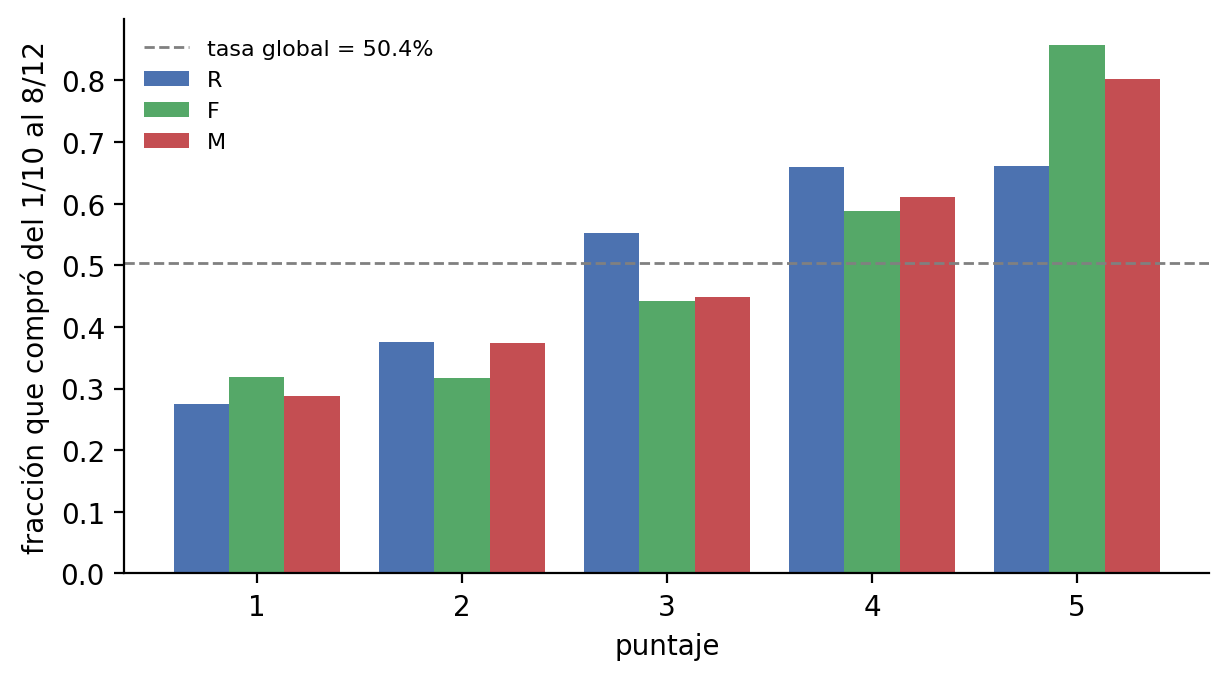
\includegraphics[width=0.75\textwidth]{p6_tasas.png}
  \caption{Tasa de compra en la ventana de prueba por puntaje de R, F y M.}
  \label{fig:p6_tasas}
\end{figure}

Las tres dimensiones ordenan bien: la tasa de compra crece con el puntaje en
las tres. Pero no separan igual.
\begin{itemize}
  \item \textbf{F separa mejor}: del 31.7\% en los puntajes bajos al 85.7\% en
    el puntaje 5, el rango más amplio, y el mayor AUC de las tres variables
    crudas, 0.721. Quien ya compró muchas veces vuelve a comprar.
  \item \textbf{M} queda muy cerca (de 28.8\% a 80.2\%, AUC 0.710). Es
    natural: un cliente que compra muchas veces acumula más monto, así que M
    y F miden en buena parte lo mismo.
  \item \textbf{R} es la que menos separa (AUC 0.674). Distingue bien entre
    los puntajes bajos (27.5\% en el 1, 55.2\% en el 3), pero se satura
    arriba: los puntajes 4 y 5 tienen la misma tasa (65.9\% y 66.1\%). Haber
    comprado hace dos semanas o hace seis no hace diferencia en una ventana
    de diez semanas que además es la temporada alta, cuando incluso los
    clientes menos recientes vuelven.
  \item \textbf{La suma de los tres puntajes} tiene el mejor AUC, 0.735,
    pero apenas por encima de F sola: combinar las tres dimensiones agrega
    poco, porque están muy correlacionadas.
\end{itemize}
Un AUC de 0.72 significa que, si se toma al azar un cliente que compró y uno
que no, F le da el valor más alto al que compró el 72\% de las veces: útil,
pero lejos de una predicción segura.

\subsection{Inciso 6.4: los campeones}

Los clientes con puntaje 4 o 5 en las tres dimensiones son \textbf{792, el
21.7\% de los clientes}. Entre el 1 de octubre y el 8 de diciembre
\textbf{generaron el 53.5\% de la venta neta} de todos los clientes con
\texttt{CustomerID}, incluidos los nuevos: \pounds1.28 millones de
\pounds2.40 millones (tabla~\ref{tab:p6_grupos}). El 81.2\% de los campeones
compró en esa ventana. Es la concentración típica de un negocio mayorista: uno
de cada cinco clientes trae más de la mitad del dinero. Para una tienda, saber
quiénes son vale más que cualquier pronóstico de la serie agregada.

\begin{table}[H]
  \centering
  \small
  \tabla{p6_grupos}
  \caption{Reparto de la venta neta del 1 de octubre al 8 de diciembre de 2011
  entre los clientes con \texttt{CustomerID}. ``Clientes con movimiento'' es
  cuántos clientes de cada grupo tuvieron alguna transacción en la ventana.
  Un cliente es nuevo si no tiene ninguna factura de venta antes del 1 de
  octubre.}
  \label{tab:p6_grupos}
\end{table}

\subsection{Inciso 6.5: los clientes nuevos}

De los 2\,596 clientes con movimiento entre el 1 de octubre y el 8 de
diciembre, \textbf{723 son nuevos}: no tienen ninguna factura de venta antes
del 1 de octubre. Generaron \textbf{el 15.7\% de la venta neta} de la ventana,
\pounds377\,860 (tabla~\ref{tab:p6_grupos}).

\paragraph{¿Puede un RFM pronosticar esa venta?} No, ni el RFM ni ningún
modelo construido cliente por cliente. Un modelo así solo puede pronosticar a
los clientes que tiene en su tabla, y un cliente nuevo no tiene fila: no hay R,
ni F, ni M que calcular, porque todavía no ha hecho nada. Lo más que puede
hacer un modelo por cliente es predecir que los clientes conocidos dejen de
comprar; nunca que aparezcan clientes desconocidos. Ese 15.7\% es un error
estructural, que no se corrige con un mejor modelo. Y es un mínimo: la venta
sin \texttt{CustomerID}, el 15.4\% de toda la venta según el inciso 1.2(f),
tampoco la ve ningún modelo por cliente.

\paragraph{Conexión con la Parte 5 y con el Proyecto 1.} En el vocabulario de
FPP2 (§10.3--10.4), la Parte 5 es un pronóstico \emph{top-down}: se
pronostica directamente la venta total. Un modelo que sume pronósticos cliente
por cliente sería \emph{bottom-up}. Solo el \emph{top-down} puede ver a los
clientes nuevos. No los ve como individuos, sino como parte del nivel de la
serie: la llegada de cientos de clientes nuevos en el cuarto trimestre es una
de las razones por las que la venta se duplicó desde septiembre, y es
justamente ese cambio de nivel el que S2 siguió y le dio la victoria en el
inciso 5.3. El \emph{bottom-up}, en cambio, empieza con una desventaja: aunque
pronosticara perfecto a cada cliente conocido, se quedaría corto en al menos
un 15.7\% de la venta con cliente. Para la comparación que pide el Proyecto 1,
esto significa que un pronóstico cliente por cliente necesita un componente
aparte para la venta de clientes nuevos (que tendría que ser de algún modo
\emph{top-down}), o va a perder contra la serie agregada en cualquier periodo
en que la tienda gane clientes, como en la temporada navideña.


\begin{thebibliography}{9}

\bibitem{chen_datos}
  D. Chen. \emph{Online Retail} [conjunto de datos].
  UCI Machine Learning Repository, 2015.
  \url{https://archive.ics.uci.edu/dataset/352/online+retail}

\bibitem{chen_rfm}
  D. Chen, S. L. Sain y K. Guo. ``Data mining for the online retail industry:
  A case study of RFM model-based customer segmentation using data mining''.
  \emph{Journal of Database Marketing \& Customer Strategy Management}
  19.3 (2012), pp.~197--208.

\bibitem{fpp2}
  R. J. Hyndman y G. Athanasopoulos. \emph{Forecasting: Principles and
  Practice}, 2a ed. OTexts, Melbourne, 2018.
  \url{https://otexts.com/fpp2/}

\bibitem{tsay}
  R. S. Tsay. \emph{Analysis of Financial Time Series}, 2a ed. Wiley, 2005.

\end{thebibliography}

\end{document}
